\chapter{混部场景导向的调度定制研究}\label{chap:sched_policy}

% Core调度框架定制(静态) -> Control Tower任务调度框架定制(动态) -> 资源感知调度机制定制(动态) -> 资源感知调度策略定制(动态) 

为解决不同混部场景下任务调度机制的不足,本章主要展开混部场景导向的定制任务调度机制研究。首先,从内核任务调度的相关配置上,针对不同应用的需求,设计了响应度优先与吞吐量优先两种基础内核配置,随后,在Sched Ext项目的基础上设计场景导向的Control Tower任务调度框架,并在此基础上结合eBPF的监测能力,进一步设计了CPU资源感知与网络资源感知的任务调度策略。

\section{内核调度配置定制}

Linux调度子系统提供了一些编译配置选项,用以针对场景进行优化,相关配置选项围绕时钟中断与抢占模型展开。

时钟中断是驱动Linux抢占式调度的核心机制,如表~\ref{tab:config_hz}所示,Linux内核提供了时钟中断频率与时钟中断处理模式两方面的配置。其中,中断的频率配置决定了调度滴答的周期,Linux提供了从100、250、300到1000四种不同的中断频率配置。越高的时钟中断频率意味着系统的整体响应度更好,同时,越高的时钟中断频率意味着更准确的时间记账。Linux在时钟中断处进行时间记账,但实际运行过程中,由于中断间隔可能存在任务切换,因此时间记账并不一定准确。时钟中断频率决定了时间片的最小粒度,而越高的时钟中断频率意味着越小的时钟中断间隔,同时在间隔中发生任务切换的概率也会越小,从而能够实现更准确的时间记账。

\begin{table}[H]
    \bicaption{\quad 内核时钟中断配置选项}{\quad Kernel clock interrupt configuration options}% caption
    \label{tab:config_hz}
    \footnotesize% fontsize
    \setlength{\tabcolsep}{4pt}% column separation
    \renewcommand{\arraystretch}{1.25}% row space 
    \centering
    \begin{tabular}{lc}
        \hline
        配置名称 & 描述 \\
        \hline
        HZ\_100  & 配置时钟中断频率为100  \\
        HZ\_250  & 配置时钟中断频率为250 \\
        HZ\_300  & 配置时钟中断频率为300 \\
        HZ\_1000 & 配置时钟中断频率为1000 \\
        HZ\_PERIODIC & 永远不要忽略时钟中断 \\
        NO\_HZ\_IDLE & 忽略空闲CPU上的时钟中断 \\
        NO\_HZ\_FULL & 忽略空闲CPU,以及只有一个可运行任务CPU上的时钟中断 \\
        \hline
    \end{tabular}
\end{table}

时钟中断会打断当前任务的执行,并产生上下文切换的开销。Linux内核提供了如表~\ref{tab:config_hz}所示的不同时钟中断处理模式来减少特定场景中不必要的时钟中断开销。在开启NO\_HZ选项之后,Linux内核允许指定部分CPU核心为NO\_HZ核心,这些CPU核心会根据不同的时钟中断处理模式调整对时钟中断的处理,如在CPU空闲时、队列中只有一个任务时忽略时钟中断。合理的NO\_HZ配置能够实现节能及减少对任务干扰的效果。

抢占通常指高优先级任务打断低优先级任务的执行。Linux内核中用户态任务总是会被中断抢占,而内核态任务则存在不同的处理。早期Linux内核实现中会在执行内核态代码时屏蔽中断,而一些较长的内核态代码会引发系统整体响应度的下降。而为提供更好的响应度,Linux在后续迭代中设计了如表~\ref{tab:config_preempt}所示的四种抢占模型,用于配置内核态代码执行时中断的处理模式。不同抢占模式的主要区别在于可被抢占位点的数量。内核代码中可被抢占的位点越多系统的实时性通常就会越好,但也意味着任务的执行更容易被打断,需要根据部署应用的不同特性来选择。

\begin{table}
    \bicaption{\quad 内核抢占模式配置选项}{\quad Kernel preemption mode configuration options}% caption
    \label{tab:config_preempt}
    \footnotesize% fontsize
    \setlength{\tabcolsep}{4pt}% column separation
    \renewcommand{\arraystretch}{1.25}% row space 
    \centering
    \begin{tabular}{lc}
        \hline
        配置名称 & 描述 \\
        \hline
        PREEMPT\_NONE  & 内核代码保持执行直到主动放弃CPU  \\
        PREEMPT\_VOLUNTARY  & 开启了内核代码中的抢占位点 \\
        PREEMPT  & 提供更多的内核代码抢占位点,实现完全抢占 \\
        PREEMPT\_RT & 进一步修改内核代码的实现,如锁机制,实现实时可抢占性 \\
        \hline
    \end{tabular}
\end{table}

时钟中断和抢占模式配置共同决定了Linux调度子系统的整体响应度,根据应用的不同需求,本文设计了响应度优先与吞吐量优先两种基本的调度子系统配置。其中,响应度优先配置使用更高的HZ与激进的抢占模式来提升整体响应度,满足应用对于延迟与实时性的需求。吞吐量优先配置则使用较低的HZ与保守的抢占模式,让CPU更多地执行任务而不是处理时钟中断,满足应用对于吞吐量的需求。

\section{Control Tower任务调度框架设计}

% 混部Linux优先级机制的问题
% - 调度队列优先级问题: 
%  - 优先级机制用于限制不同任务对CPU时间的使用,并不能保证高优先级的应用一定能够比低优先级应用优先调度
% - 调度类优先级问题:
%  - 运行在实时调度类中的LC任务如配置不当,一方面不利于应用性能,另一方面容易造成系统崩溃
%  - 将低优先级的任务允许在Idle类是嵌入式领域的常用做法,但不够灵活,且违背Linux设计语义
% 解决方式
% - 引入Ext调度类,使能调度队列隔离
% - 利用BPF Scheduler的灵活性
% 调度器架构
% - User Input: Task define, Resource define
% - eBPF Input: Task status, Resource status
% - Control Signals: BPF Map、BPF Prog: rodata\bss
% - BPF Scheduler: Select Eligible Task to Eligible CPU
% - Control: BPF Helper \ User Define Command \ eBPF Define
% 调度模式
%  - 全局调度
%  - Per-CPU调度
% 调度策略
%  - FIFO
%  - RR
%  - Vtime

混部场景中,为高优先的应用设置更高的优先级是保障应用QoS的一种途径。Linux调度子系统中提供了调度类与调度队列两层的优先级定义,但在保障应用QoS上两层优先级都存在一定的不足:

\begin{itemize}

    \item 在调度类层,利用调度类的优先级差异能够保证高优先就绪时总能抢占低优先应用。具体实践中可将高优先应用添加到较高优先级的调度类,或将低优先应用添加到低优先级调度类实现。将高优先应用添加到高优先级调度类时,需要充分考虑应用的特点与高优先级调度类的参数配置,不当的配置不仅会影响应用本身的性能,还有可能引发整个系统性能下降。将低优先任务添加到低优先级调度类时,需要考虑一定的风险。例如,将低优先任务添加到Idle调度类。首先,将常规任务放置到Idle调度类这一操作破坏了Idle调度类的设计语义,不利于系统能耗的优化。其次,Idle调度机制在实现上十分简单,难以满足多样的调度需求,无法有效地进行QoS保障。

    \item 在调度队列层,以CFS调度器为例,Linux提供了从-20到20的静态优先级,对应调度实体vruntime的不同积累速度。在Run Queue中,高优先级的应用vruntime积累相对缓慢,从而获取更多的调度机会。但是随着vruntime不断累积,高优先应用仍存在在被低优先应用抢占的可能。除此之外,CFS调度器中还有许多启发式逻辑影响到高优先应用的QoS。例如,CFS调度器会为每个Run Queue维护一个基准vruntime,并赋予给新创建或新唤醒的进程。基准vruntime被设置为Run Queue中vruntime的最小值,使得新创建或新唤醒的应用总是能够优先被执行。这一启发式逻辑没有考虑到进程之间的优先级,当低优先级大量唤醒或创建时,高优先应用反而会因频繁抢占产生QoS劣化。其次,调度队列层优先级无法跨CPU产生作用,一方面会导致高优先应用与运行在其他CPU上的低优先应用争抢资源,另一方面也使得应用在不同CPU上迁移时,相对优先级变化导致优先性丧失。

\end{itemize}

优先级机制上的缺陷导致Linux难以在混部场景中有效地进行QoS保障,同时Linux内核调度在开发、部署于迭代上十分困难。而为解决这些问题,本文首先设计了Control Tower任务调度框架,支持灵活的调度策略设计并提供友好的调度策略开发方式。Control Tower任务调度框架基于Sched Ext项目实现。引入Sched Ext项目,一方面,支持使用BPF技术来定制调度策略,并借助Ext调度类插件化的特性优化调度策略的开发流程。另一方面,利用Ext调度类构造调度类优先级差异,既能够实现根据场景量身定制调度策略,又不会破坏现有调度子系统的设计。

Control Tower任务调度框架如图~\ref{fig:bpf_scheduler_arch}所示,其中核心是BPF调度策略,能够通过Sched Ext项目提供的接口来定制Ext调度类的调度行为。同时,Control Tower任务调度框架允许向BPF调度策略引入额外的数据输入源,包括用户与其他子系统的数据输入。这些额外的输入数据通过BPF Map等数据共享机制提供给BPF调度策略,并辅助进行调度决策。此外,Control BPF调度框架也允许BPF调度策略与用户态程序协作,来实现更灵活的调度机制设计。

\begin{figure}[H]
    \centering
    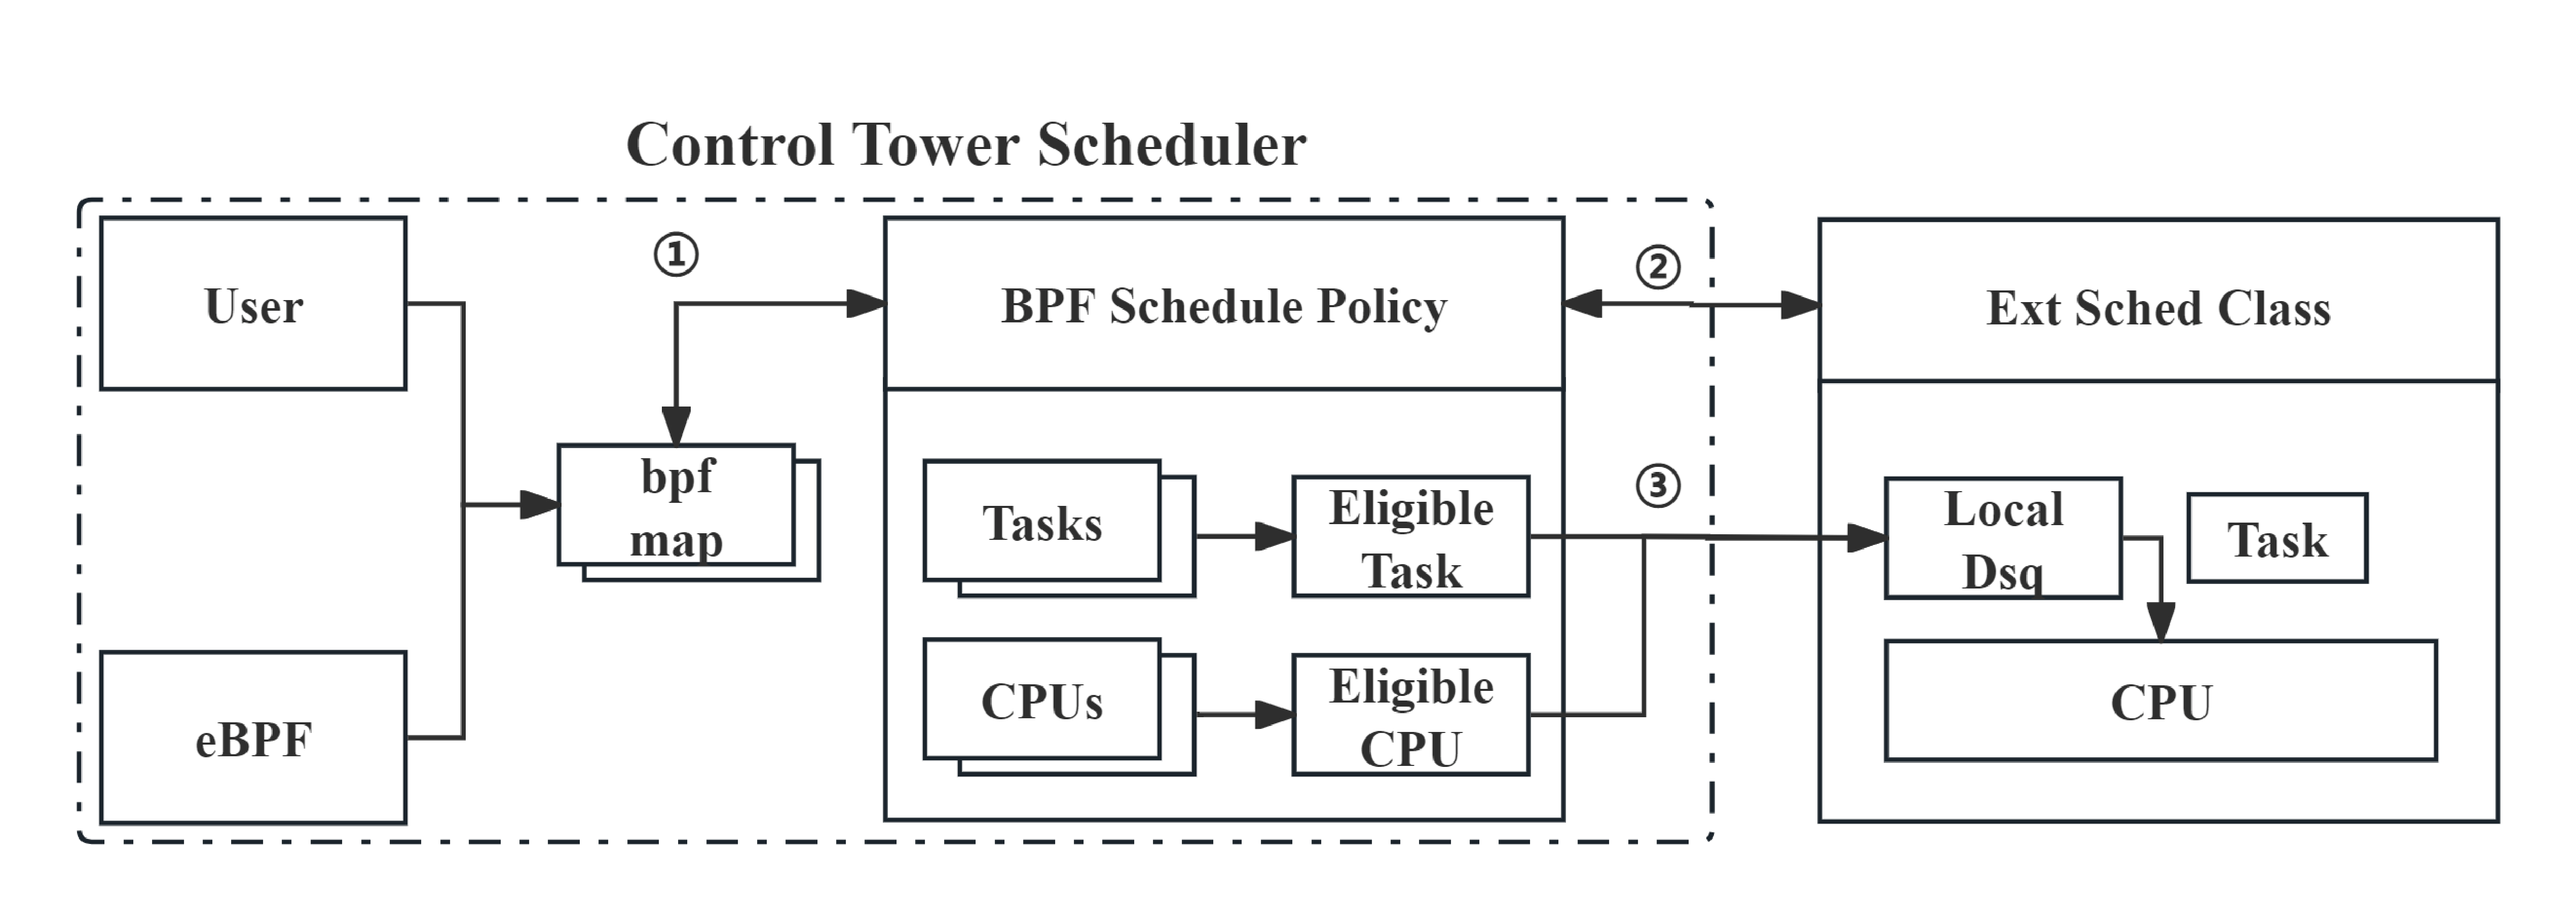
\includegraphics[width=0.8\textwidth]{bpf_scheduler_arch}
    \bicaption{\quad Control Tower任务调度框架设计}{\quad Control Tower task scheduling framework design}
    \label{fig:bpf_scheduler_arch}
\end{figure}

用户与eBPF外部数据源区别于Ext调度类提供的调度信息,可由用户自定义或从其他子系统中采集。其中,用户数据源作用在BPF调度策略初始化和运行时。初始化时,用户可定义CPU资源拓扑、BPF调度策略参数等,并通过修改BPF程序的rodata、bss段来将静态信息传递给BPF调度策略。策略运行时,用户程序可通过读写BPF调度策略预先声明BPF Pin Map来与BPF调度策略交互,如传递用户对进程、Cgroup的优先级、类型、资源需求等声明。eBPF外部数据源基于其他子系统中插桩实现,包括内核资源分配、系统调用等关键路径上,这些数据可直接通过BPF Map共享给BPF调度策略,同时,在不同的混部场景中,eBPF插桩也可以根据需要自由选择与定制。

BPF调度策略既可以直接定制Ext调度行为,也可以在调度过程中利用上述的额外数据源来调整调度行为。同时,BPF调度策略也可以通过BPF Map来将调度信息共享给用户程序与其他子系统,从而利用用户程序的灵活性以及eBPF对如网络子系统的定制能力。此外,Control Tower任务调度框架还提供了两种基本调度模式和三种基本调度策略来辅助BPF调度策略的开发。 

在调度模式上,Control Tower任务调度框架支持如图~\ref{fig:bpf_sched_mode}所示的Per-CPU调度与全局调度两种调度模式。其中,Per-CPU调度是Linux中常用的调度模式,核心在于将调度卸载到各个CPU上来避免共享内存导致的竞争。如图~\ref{fig:bpf_per_cpu}所示,BPF调度框架中通过为每个CPU创建一个BPF DSQ,并将调度策略限制在本地CPU的BPF DSQ上来实现Per-CPU调度。Per-CPU调度模式适用于CPU数量较多且对调度开销要求较高的场景。在延时敏感的混部场景中,将调度延时降低到应用的延时阈值内是保障QoS的一种方式,受限于内核的HZ配置,Per-CPU调度延时最小为1ms(1000HZ),同时,由于Linux HZ配置是全局的,而较高的时钟中断会导致整个系统中时钟中断处理的资源使用增大,影响CPU敏感任务的执行。而为解决调度延时的问题,Control Tower任务调度框架提供了全局调度模式。如图~\ref{fig:bpf_global}所示,全局调度模式基于全局调度队列与高精度时钟实现,与其他研究类似,首先选择一个CPU作为调度核心,并在这个CPU上创建全局的DSQ。同时,在调度核心上设置一个BPF Timer,利用高精度时钟实现ns级的调度周期。全局调度模式的调度过程中,首先将新创建的任务加入到全局DSQ上,每次BPF Timer的回调中,调度核心会更新任务的记账信息并尝试调度任务,并抢占时间片耗尽的任务,其中调度核心与其他核心的交互通过IPI实现。

\begin{figure}[!htbp]
    \centering
    \begin{subfigure}[b]{0.45\textwidth}
        
\includegraphics[width=\textwidth]{bpf_per_cpu}
        \caption{Per-CPU调度模式}
        \label{fig:bpf_per_cpu}
    \end{subfigure}
    \hspace{0.5cm}
    \begin{subfigure}[b]{0.45\textwidth}
        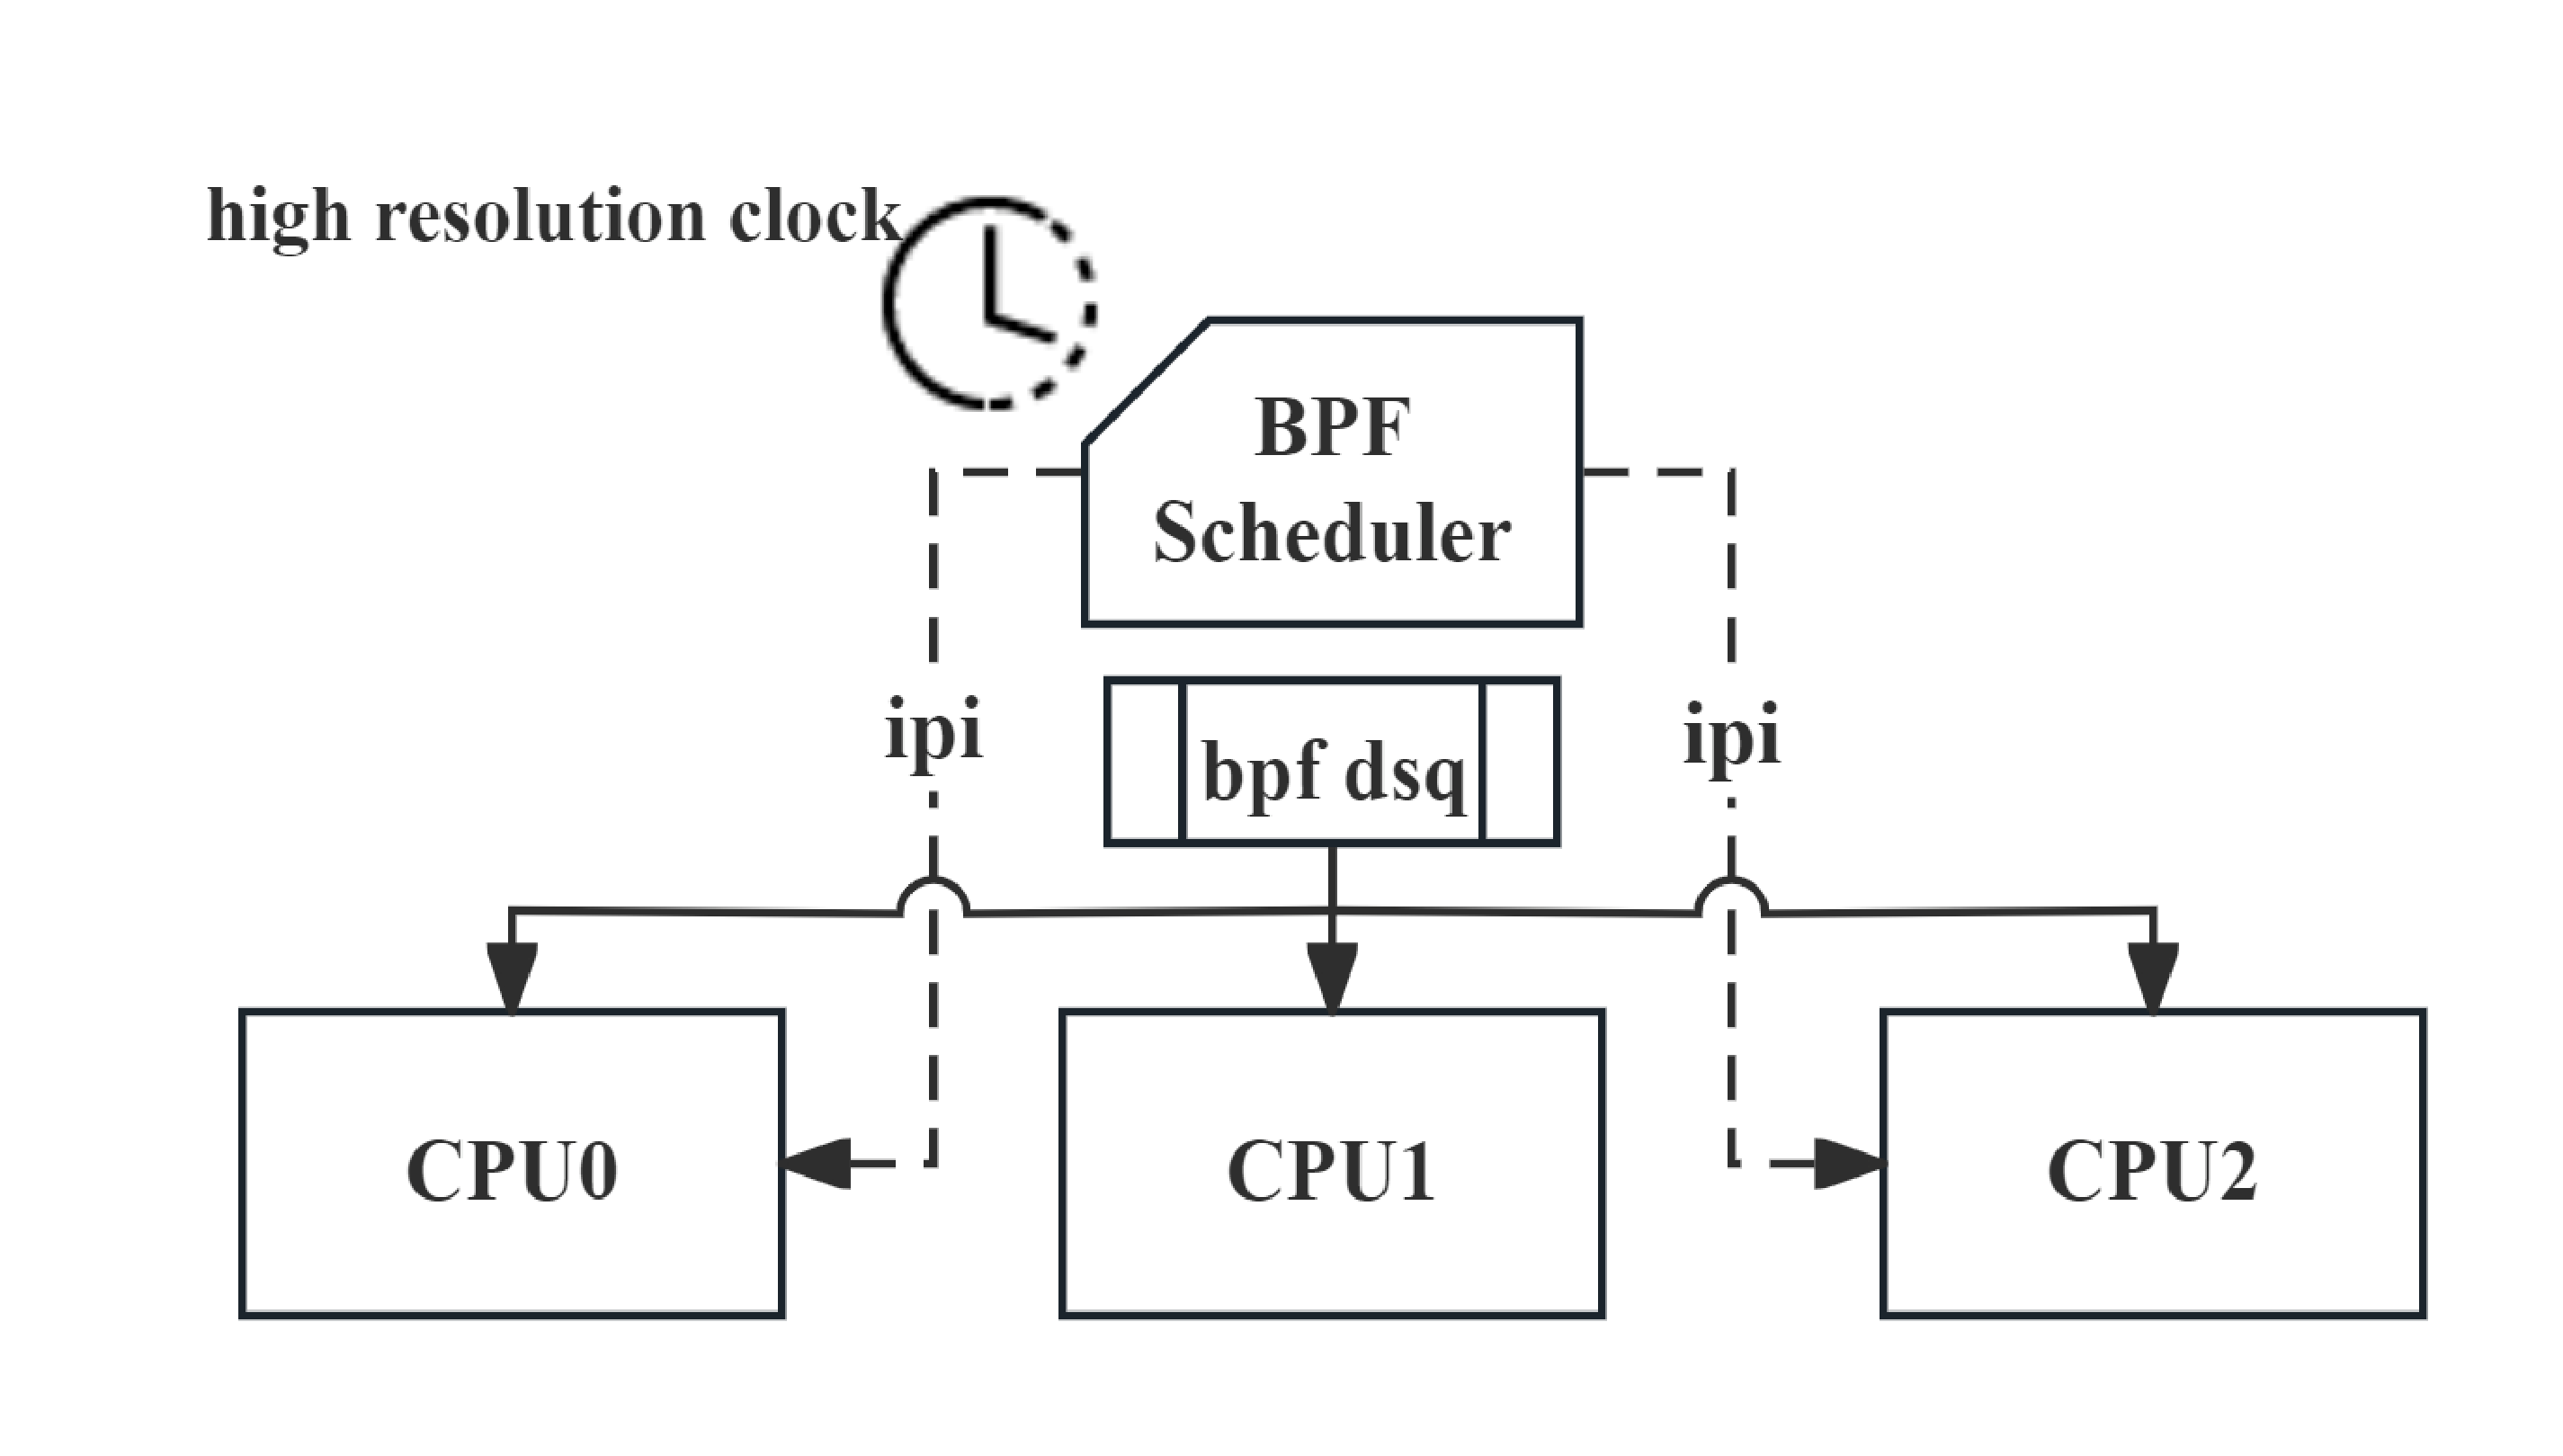
\includegraphics[width=\textwidth]{bpf_global}
        \caption{全局调度模式}
        \label{fig:bpf_global}
    \end{subfigure}
\bicaption{\quad Control Tower任务调度模式}{\quad Control Tower task scheduling mode}
\label{fig:bpf_sched_mode}
\end{figure}

在调度策略上,Control Tower任务调度框架提供了三种基本的调度策略实现:

\begin{enumerate}
    \item \textbf{基于FIFO的非抢占式调度}:BPF调度策略中使用FIFO DSQ,并设置每个入队任务的时间片为无限,任务运行直到主动退出,随后BPF调度策略取出下一个任务执行。
    
    \item \textbf{基于RR的抢占式调度}:BPF调度策略中使用FIFO DSQ, 并按照配置设置每个入队任务的时间片,每次时钟滴答时检查当前任务的剩余时间片,抢占时间片耗尽的任务并切换到下一个任务执行。

    \item \textbf{基于vtime的抢占式调度}:BPF调度策略中使用vtime DSQ,vtime DSQ按照vtime大小对任务进行排序,初始时设置每个入队任务的初始vtime,并在每个时钟滴答里根据任务的静态优先级更新vtime,并进行抢占判断。当抢占发生时,vtime越小的任务越优先被调度。
\end{enumerate}

本文在Control Tower任务调度框架的实现中,包括使用C语言编写的约1500行代码以及在Ext调度类上约200代码的修改。相较于Linux任务调度机制,Control Tower任务调度框架能够提供更灵活的任务调度机制与调控手段,并通过定制和组合不同的外部数据来源、调度模式与调度策略来满足不同混部场景应用对调度机制的需求,以更好地保障高优先应用的QoS。

\section{Control Tower资源感知任务调度}

% 对于CPU资源的隔离,常见的方式是显示地隔离不同应用能够使用的CPU,这种静态的划分方式并不能有效的使用资源,而在本章中提出了基于BPF调度器的调度队列隔离,高低优先级的应用在调度队列优先级机制之上共享相同CPU,使得高优先级应用运行时总是能够优先地使用CPU资源。

% 其次,相较于常见的调度类隔离,本章基于BPF调度器实现更为灵活,通过结合eBPF强大的监测能力,让BPF调度器感知高优先级应用CPU资源、网络资源的使用,而通过设置相关的资源约束,从而结合不同高优先级应用的资源使用特征与调度目标,更充分的利用资源。

\subsection{CPU资源感知的任务调度} 

% 进行CPU资源隔离的原因
% CPU Set静态资源划分的问题
% CPU资源感知机制的实现
% - 用户定义的CPU拓扑
% - Ext调度类eBPF hook
% CPU资源感知策略的实现
% - 保守调度场景
% - SMT场景 

CPU拓扑描述了CPU之间的资源共享情况,而CPU之间的资源共享是混部场景中“吵闹邻居”的核心原因,这要求调度需要考虑CPU间的拓扑关系。使用CPU Affinity机制将不同应用划分到不同的CPU集合中是常用方式,然而这种方式存在一些缺陷。首先,CPU Affinity隔离粒度较粗,划分不当容易造成CPU资源浪费。其次,静态的CPU集合划分没有考虑到应用CPU资源使用的动态特性,较保守的策略容易造成资源浪费,而激进的策略则容易引发QoS劣化。

造成上述问题的核心在于划分CPU集合时并没有考虑到不同应用对CPU资源的实际使用情况,而为解决这一问题,本文设计了CPU资源感知的任务调度策略,调度逻辑如伪代码~\ref{alg:cpu_aware_sched}所示,通过增加外部数据源的方式,让低优先任务感知高优先应用使用CPU资源的情况,并结合用户输入的CPU拓扑判断是否需要出让CPU资源,从而实现高优先应用的QoS保障。

CPU资源感知的任务调度策略基于Control Tower任务调度框架实现,包含约250行eBPF代码。首先,在BPF程序初始化时,用户需要传入当前系统CPU拓扑以及低优先任务所能使用的CPU数量。随后,BPF程序初始化过程中会创建一个全局数组记录Ext调度类所管理的CPU状态,并通过在Ext调度类cpu\_acquire与cpu\_release处的插桩动态更新。任务调度时,BPF调度策略读取全局数组,计算得到当前低优先任务能够使用的CPU数量,并与阈值进行比较。当不满足CPU阈值时,拒绝进行任务调度,而目标CPU会在Local DSQ没有任务执行时,出让CPU并被Idle调度类抢占。而当CPU满足阈值时,BPF调度策略首先将任务调度到目标CPU的Local DSQ上,并根据目标CPU的状态来决定是否需要发送IPI。

\begin{algorithm}[H]
    \caption{Pseudocode for CPU resource-aware task scheduling}
    \label{alg:cpu_aware_sched}
    \begin{algorithmic}[1]
    
    \Function{cpuAcquire} {cpu}
    \State Insert cpu to CPU\_Map;
    \EndFunction
    
    \Function{cpuRelease} {cpu}
    \State Remove cpu from CPU\_Map;
    \EndFunction
    
    \Function {schedule}{}
        \While{True}
            \If{$\text{CPU\_Acquired + CPU\_Idle} < \text{CPU\_Available}$ }
                \State Set Exclusive Flag;
                \For{each no\_hz core C}
                    \State Send an IPI to envoke target CPU rescheduling.
                \EndFor
                \State Yield to higher priority scheduler class;
            \EndIf
            \State Remove Exclusive Flag;
            \State Dispatched tasks;
        \EndWhile
    \EndFunction
    \end{algorithmic}
\end{algorithm}

Control Tower任务调度框架提供了以调度队列为粒度的CPU资源划分,相较于CPU Affinity粒度更细。借助调度类优先级差异,低优先任务能够在高优先任务运行时及时出让CPU资源,从而实现动态的CPU资源分配。然而这种资源的出让没有考虑CPU的拓扑关系,在如SMT作为底层硬件的混部场景中,无法有效地保障高优先应用的QoS。而CPU资源感知任务调度策略通过用户输入以及CPU资源的eBPF探测弥补了这一缺陷,能够更好地在SMT以及激进的高优先任务QoS保障场景中发挥作用。

\subsection{网络资源感知的任务调度}

% 网络资源感知的目标
% - 现有问题
% 网络资源感知机制的实现
% - Epoll系统调用eBPF hook
% - LC应用划分
% 网络资源感知策略的实现
% - LC应用低负载,高负载,负载高时,基于Epoll的LC应用特征变化(CPU敏感),要求吞吐量
% - 交还eevdf, 动态时间片

混部场景中LC应用通常为网络服务应用,在画像分析中发现,网络服务应用的资源使用倾向与敏感度在不同负载下存在差异。在负载较低时,由于请求量少、处理时间快,因此对资源的需求不高,且受到干扰影响不明显。而在负载较高时,对资源的需求激增,同时干扰会导致处理请求的速度变慢,而待处理请求的积压会引发较大QoS劣化。

高性能网络应用通常使用epoll作为底层的网络机制。epoll允许进程同时监听多个连接,并在连接就绪时进行批量处理。相较于阻塞型网络系统调用,使用epoll能够在大量请求时减少频繁地阻塞唤醒过程,从而支持更高的并发量。epoll机制涉及到多个系统调用,而其中最为核心的是epoll\_wait系统调用。进程在注册等待事件之后,就能够通过epoll\_wait系统调用来获取当前的就绪事件。当存在就绪事件时,epoll\_wait系统调用会返回就绪的事件数量,而当没有事件就绪时,epoll\_wait仍然会阻塞进程。

实际生产环境中,网络服务应用的负载更加具有波动性,然而Linux任务调度机制并不考虑混部应用在不同负载对于调度需求,同时也缺乏有效的应用负载感知机制。为解决上述问题,本文设计了网络资源感知的任务调度策略,调度逻辑如伪代码~\ref{alg:network_aware_sched}所示。网络感知调度策略通过eBPF插桩获取应用的实时负载,并从用户输入获取目标应用在不同负载下的调度需求。调度过程中针对不同的负载地实施不同的调度策略,如在低负载下以系统吞吐为目标,而在高负载时以高优先应用的QoS保障为目标。

\begin{algorithm}[H]
    \caption{Pseudocode for network resource-aware task scheduling}
    \label{alg:network_aware_sched}
    \begin{algorithmic}[1]

    \Function {do\_epoll\_wait\_return}{$nr\_event$}
        \State Write timestamp of current epoll wait;
        \State Write $nr\_event$ of current epoll wait;
        \State Update total event count;
        \State Update count of epoll wait;
    \EndFunction

    \Function {schedule}{}
        \While{True}
            \State Read epoll wait delta from bpf map;
            \If{$\text{EPOLL\_WAIT\_DELTA} < \text{EPOLL\_WAIT\_THRESHOLD}$ }
                \State Set Exclusive Flag;
                \For{each no\_hz core C}
                    \State Send an IPI to envoke a rescheduling;
                \EndFor
                \State Yield to higher priority scheduler class;
            \EndIf
            \State Remove Exclusive Flag;
            \State Dispatched tasks;
        \EndWhile
    \EndFunction
    \end{algorithmic}
\end{algorithm}

网络资源感知调度策略增加了基于epoll\_wait系统调用探测的eBPF数据源,包含约200行eBPF代码。在具体eBPF代码中,首先会创建两个Per-CPU BPF Map,分别记录Per-CPU上epoll\_wait系统的频率与事件数量。而在观测粒度的的选择上,策略支持pid、Cgroup以及全局三种监测粒度。在eBPF插桩位点上,选择do\_epoll\_wait内核函数的返回处进行插桩。此处不仅表示一次epoll\_wait系统调用的完成,还也能够通读取返回值,获取此次epoll\_wait系统调用所得到的epoll事件数量。每次计数完毕后都会更新此次计数的时间戳,结合计数与时间戳数据就能够计算应用的负载量。

网络资源感知调度策略在Control Tower调度框架中的实现也有多种方式。首先,在低负载时,直接调度任务而不考虑CPU拓扑上的资源竞争,在满足高优先低负载时的基本延时需求的同时,实现更高的系统吞吐。而在高负载时,采用避让的原则,减少与高优先应用的资源竞争,从而实现高优先应用的QoS保障。其次,也可以将探测逻辑与调度策略分离。如在低负载时关闭BPF调度策略,此时低优先任务会被Fair调度类调度,并与高优先应用处在相同的调度队列中,通过分时复用进一步提高吞吐。而在高负载时,加载CPU资源感知的BPF调度策略,并设置较为保守的参数来优先保障高优先应用的QoS。

% \subsection{基于PMU实现的其他资源感知策略}

\section{实验设计与分析}

\subsection{实验环境}

任务调度实验在两台服务上展开,服务器硬件信息如表~\ref{tab:exp_env}所示。实验中考虑到内核兼容性与适配问题,使用Qemu 6.2.0与KVM虚拟机作为混部应用的主要运行环境。

\begin{table}[H]
    \bicaption{\quad 任务调度实验服务器硬件参数}{\quad Information about server hardware for task scheduling experiments}% caption
    \label{tab:exp_env}
    \footnotesize% fontsize
    \setlength{\tabcolsep}{4pt}% column separation
    \renewcommand{\arraystretch}{1.25}% row space 
    \centering
    \begin{tabular}{lc}
        \hline
        硬件资源 & 硬件信息 \\
        \hline
        CPU & Intel Xeon Gold 6148 (40 cores) * 2 \\
        Processor Core Frequency & 2.4GHz,Turbo 3.7 GHz \\
        L1 Caches & 32KB,  8-way set associative, split D/I \\
        L2 Caches & 1024KB, 16-way set associative \\
        L3 Caches & 28160KB, 11-way set associative \\
        Main Memory & 32GB * 8, 2666MHz DDR4 \\
        NIC & Intel Corporation Ethernet Connection X722 for 10GbE SFP+(10Gbit) \\
        \hline
    \end{tabular}
\end{table}

实验中选择Redis、Memcached、Mysql、Nginx四种LC应用和graph500、ffmpeg两种BE应用来构造混部环境,并使用stress-ng来模拟干扰。而在负载选择上,本文通过如表~\ref{tab:app_work}所示的Benchmark来生成负载,并通过预先实验确定固体虚拟机配置下的应用的最大负载值,定义为100\%工作负载。

\begin{table}[H]
    \bicaption{\quad 实验应用及负载配置}{\quad Experimental application and workload configuration}% caption
    \label{tab:app_work}
    \footnotesize% fontsize
    \setlength{\tabcolsep}{8pt}% column separation
    \renewcommand{\arraystretch}{1.25}% row space 
    \centering
    \begin{tabular}{llc}
        \hline
        应用名称 & 测试工具 & 最大负载 \\
        \hline
        Redis     & Memtier Benchmark & 60000 op\textbackslash s \\
        Memcached & Memtier Benchmark & 100000 op\textbackslash s \\
        Mysql     & TPCC              & 7000  tpmc \\
        Nginx     & wrk2              & 20000 qps \\
        Graph500  & -                 & - \\
        FFmpeg    & vbench            & - \\
        \hline
    \end{tabular}
\end{table}

\subsection{响应度优先内核性能}

响应度优先任务调度配置使用HZ\_1000配置时钟中断频率,并配置PREEMPT抢占模式。实验在4 CPU、1024MB内存的虚拟机上展开,选择Redis、Memcached、Nginx和Mysql四种延迟敏感应用来分别与stress\_ng CPU干扰应用进行混部,并与HZ\_250和VOLUNTARY抢占模式的CloudHV默认Linux内核比较。

混部实验结果如图~\ref{fig:perf_response}所示,响应度优先内核配置几乎在所有混部场景下都实现了更好的应用QoS保障。对于业务逻辑较简单的LC应用,如Redis、Memcached与Nginx,响应度优先内核分别实现降低99分位尾延迟最高39.2\%、36.9\%、35.2\%的效果。高响应度的配置能够及时地为LC应用分配CPU资源,避免请求的积压从而保障应用的延时需求。MySQL混部实验中响应度优先内核能在一定程度上提升MySQL的事务处理能力。但由于MySQL线程数多、业务逻辑复杂,在较高负载时,由于NO\_HZ核心配置多线程下失效,频繁的时钟中断也导致执行有效任务的时间减少,使得MySQL的延时上升。

\begin{figure}[H]
    \centering
    \begin{subfigure}[b]{0.32\textwidth}
      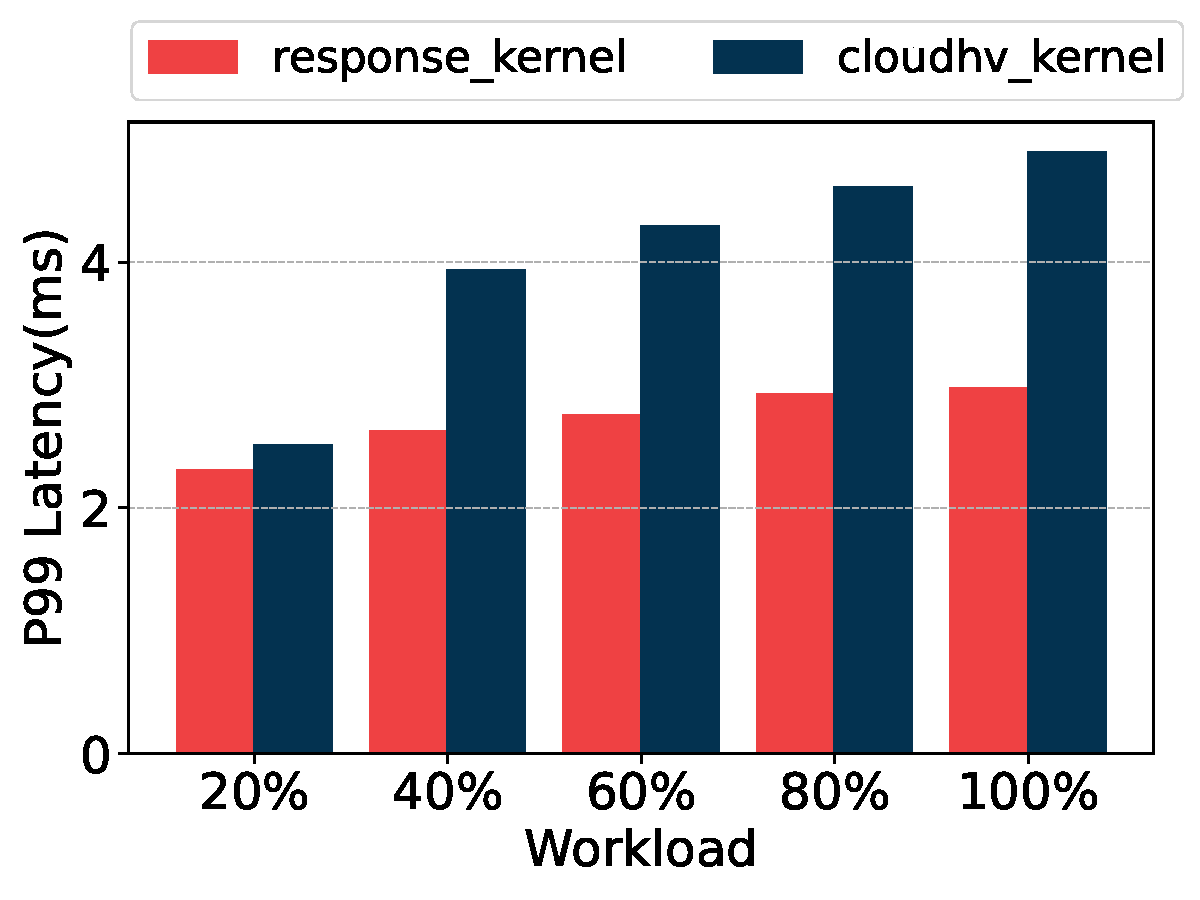
\includegraphics[width=\textwidth]{response_kernel_redis}
      \caption{Redis请求延迟}
      \label{fig:response_kernel_redis}
    \end{subfigure}
    \begin{subfigure}[b]{0.32\textwidth}
      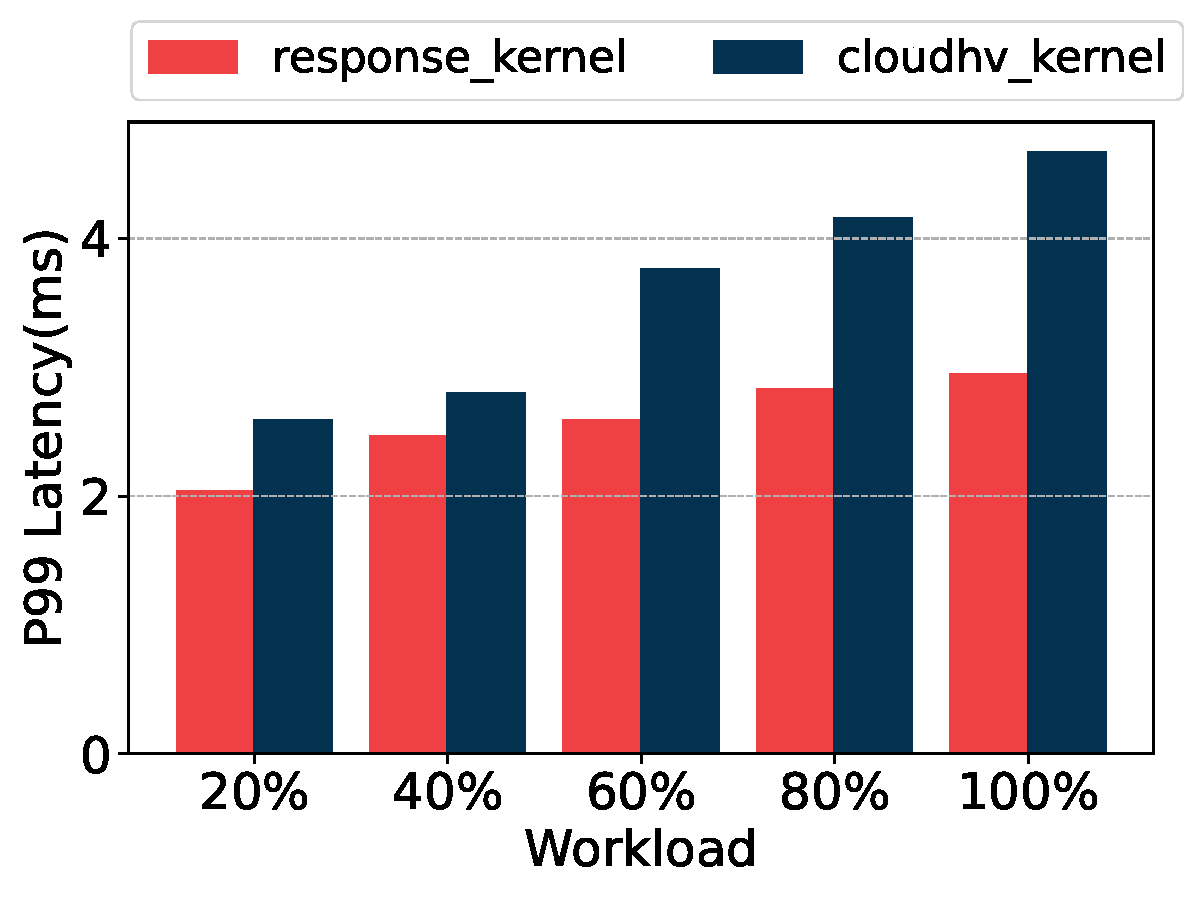
\includegraphics[width=\textwidth]{response_kernel_memcached}
      \caption{Memcached请求延迟}
      \label{fig:response_kernel_memcached}
    \end{subfigure}
    \begin{subfigure}[b]{0.32\textwidth}
        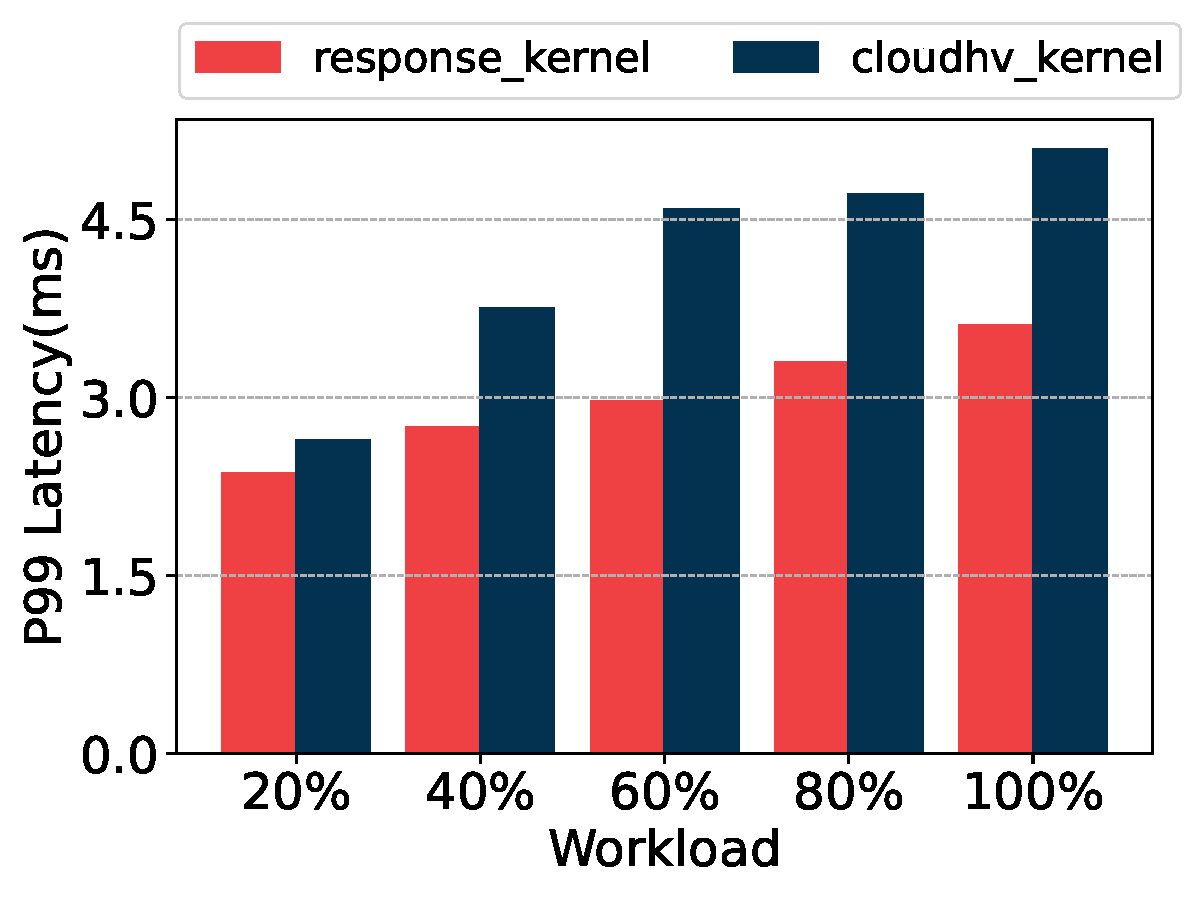
\includegraphics[width=\textwidth]{response_kernel_nginx}
        \caption{Nginx请求延迟}
        \label{fig:memcached_response}
      \end{subfigure}
      \begin{subfigure}[b]{0.32\textwidth}
        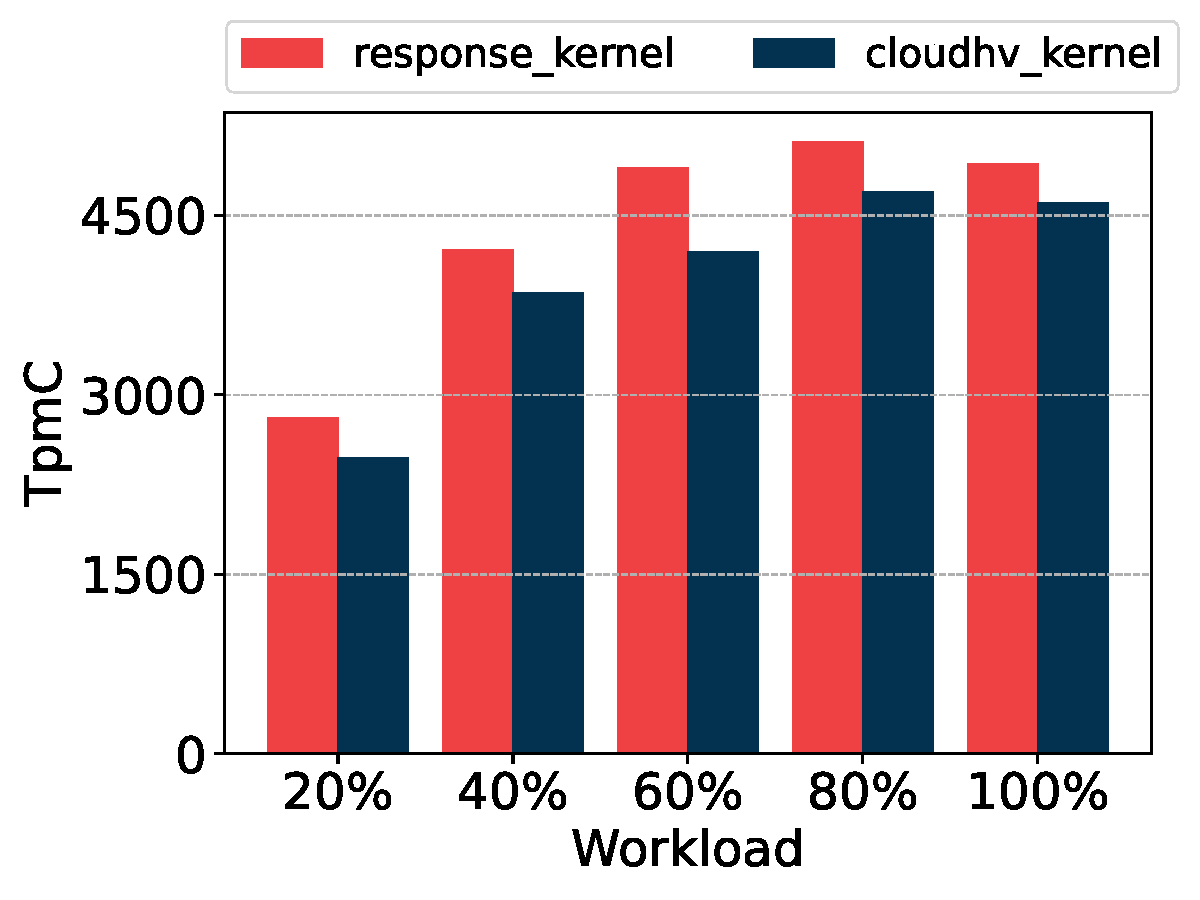
\includegraphics[width=\textwidth]{response_kernel_mysql}
        \caption{\quad MySQL每秒事务数量}
        \label{fig:memcached_response}
      \end{subfigure}
      \begin{subfigure}[b]{0.32\textwidth}
        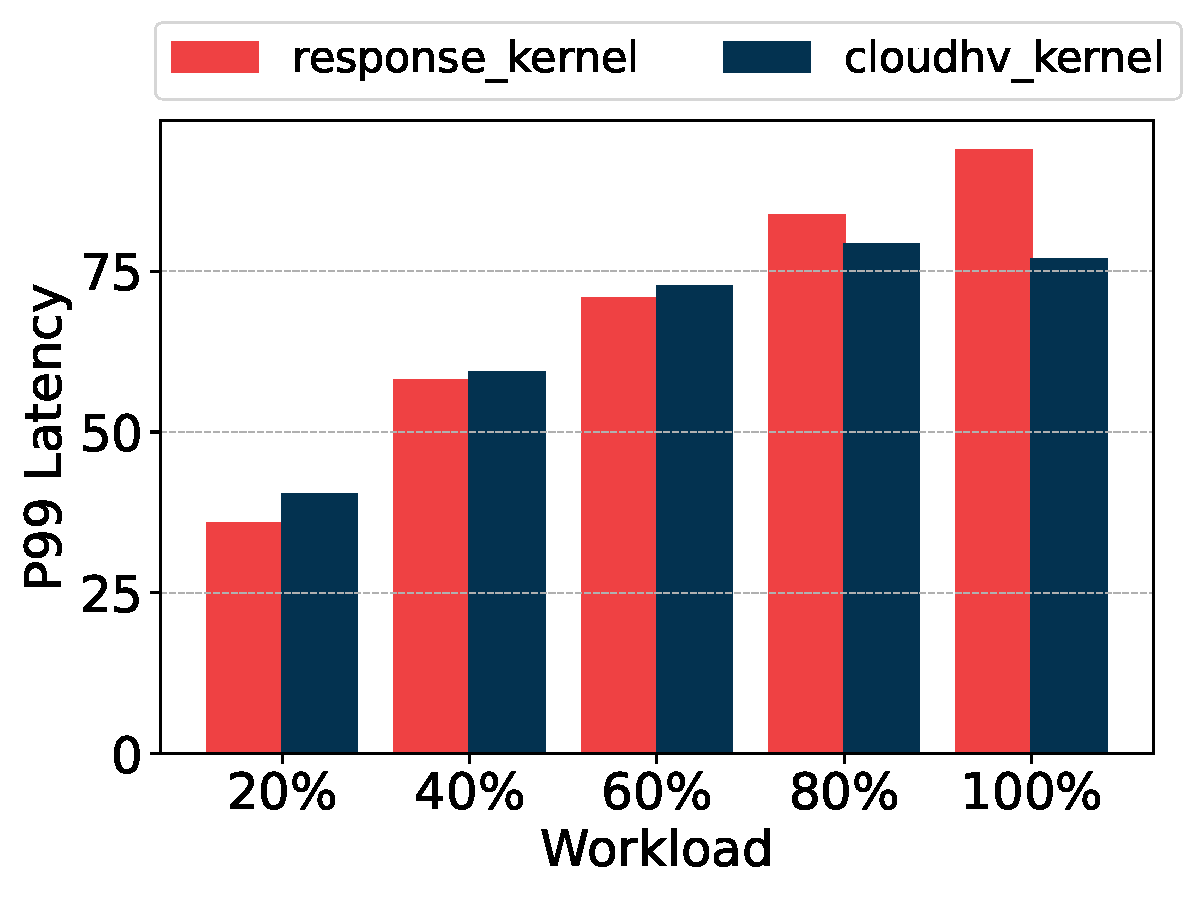
\includegraphics[width=\textwidth]{response_kernel_mysql_latency}
        \caption{MySQL请求延迟}
        \label{fig:memcached_response}
      \end{subfigure}
    \bicaption{\quad 响应度优先内核对LC应用服务性能的保障效果}{\quad Effectiveness of responsiveness-first kernel for LC application QoS}
    \label{fig:perf_response}
\end{figure}

\subsection{吞吐量优先内核性能}

% graph500(time) \ ffmpeg 

吞吐量优先任务调度配置使用HZ\_100配置时钟中断,并开启PREEMPT\_NONE抢占模式。实验在4 CPU、1024MB内存的虚拟机上展开,选择Graph500、ffmjepg两种CPU敏感型应用分别与stress\_ng CPU干扰应用混部,并与使用HZ\_250和VOLUNTARY抢占模式的CloudHypervisor默认Linux内核进行比较。Graph500主要执行图计算算法,因此执行时间是其重要的性能指标,实验中使用time工具记录进程在用户态与内核态耗费的时间,并将平均每分钟能够执行的Graph500计算数量作为性能指标。ffmpeg是主流的媒体处理工具,实验中使用vBench模拟负载并同样记录进程在用户态与内核态耗费的时间,而对于媒体处理应用而言,每秒处理帧数是其重要的性能指标。

\begin{figure}[H]
    \centering
    \begin{subfigure}[b]{0.35\textwidth}
        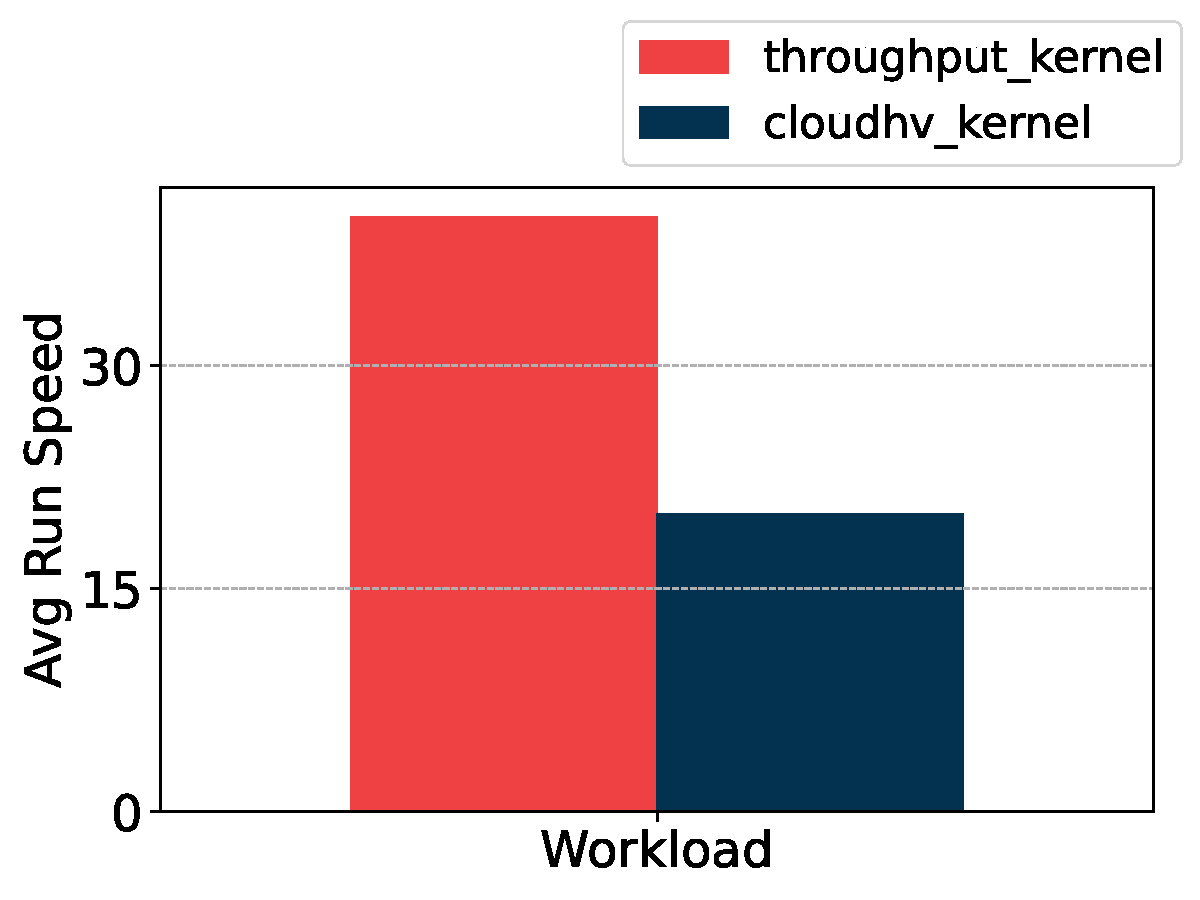
\includegraphics[width=\textwidth]{throughput_kernel_graph500_speed}
        \caption{\quad Graph500每分钟执行数量}
        \label{fig:throughput_kernel_graph500_speed}
    \end{subfigure}
    \begin{subfigure}[b]{0.35\textwidth}
        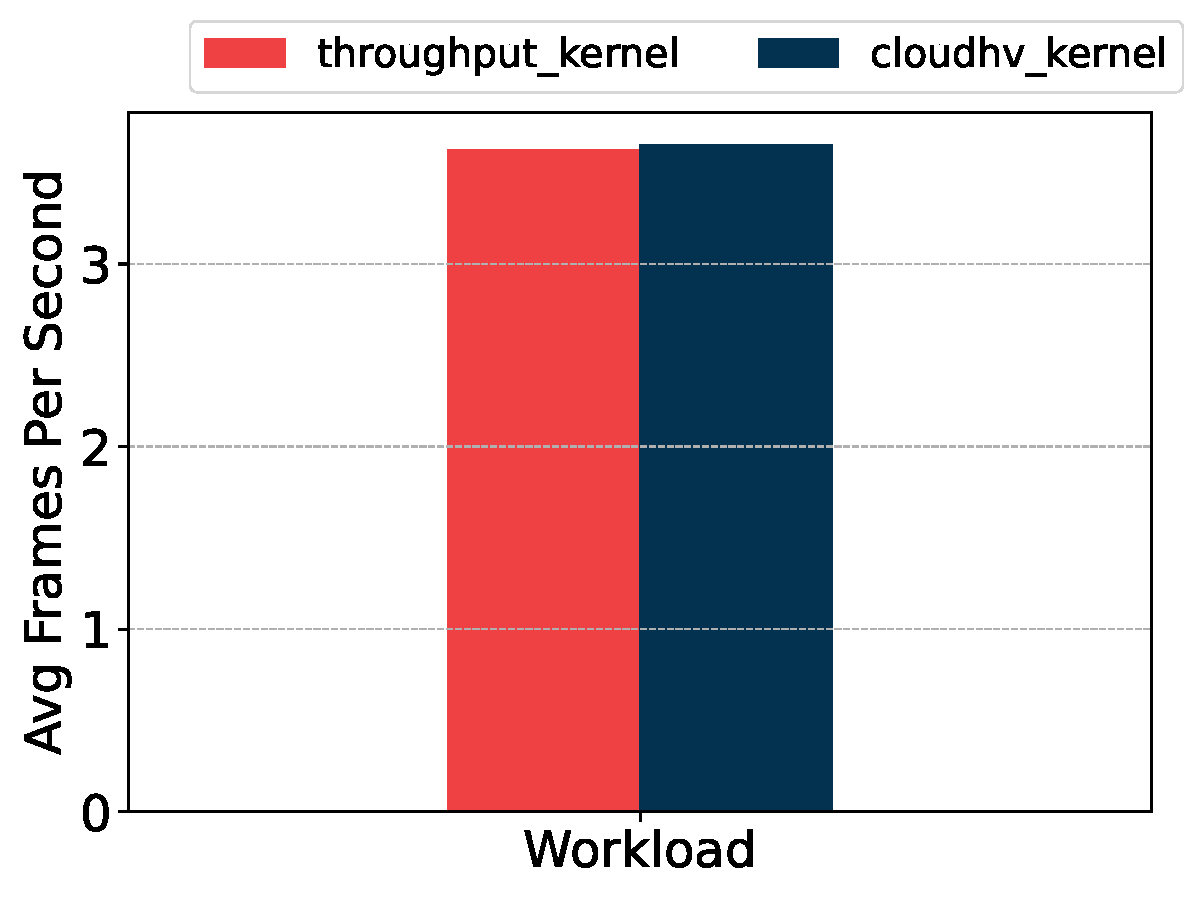
\includegraphics[width=\textwidth]{throughput_kernel_ffmpeg_speed}
        \caption{\quad FFmpeg每秒处理帧数量}
        \label{fig:throughput_kernel_ffmpeg_speed}
    \end{subfigure}
    \bicaption{\quad 吞吐量优先内核对BE应用服务性能的保障效果}{\quad Effectiveness of throughput-first kernel for BE application QoS}
    \label{fig:perf_throughput}
\end{figure}

混部实验结果如图~\ref{fig:perf_throughput}所示。对于Graph500,吞吐量优先内核实现了平均执行速度提升1.6 $\times$的效果。而在如图~\ref{fig:perf_throughput_time}所示的运行时间分布上可以看出,Graph500在吞吐量优先内核下,得益于保守的抢占模式与较低的时钟中断频率,使得在内核态运行的时间大大减少。同时,更少的上下文切换也提升了应用执行的局部性,使得Graph500在用户态的运行时间也有所减少。而对于ffmpeg,吞吐量优先内核与CloudHV默认内核的差异并不明显。这是因为不同于Graph500,ffmpeg在运行过程中需要频繁进行IO来读取媒体文件,因此等待IO的时间更多,此时即便设置更小的时钟中断频率,但对于提升应用性能上意义并不大。

\begin{figure}[H]
    \centering
    \begin{subfigure}[b]{0.35\textwidth}
        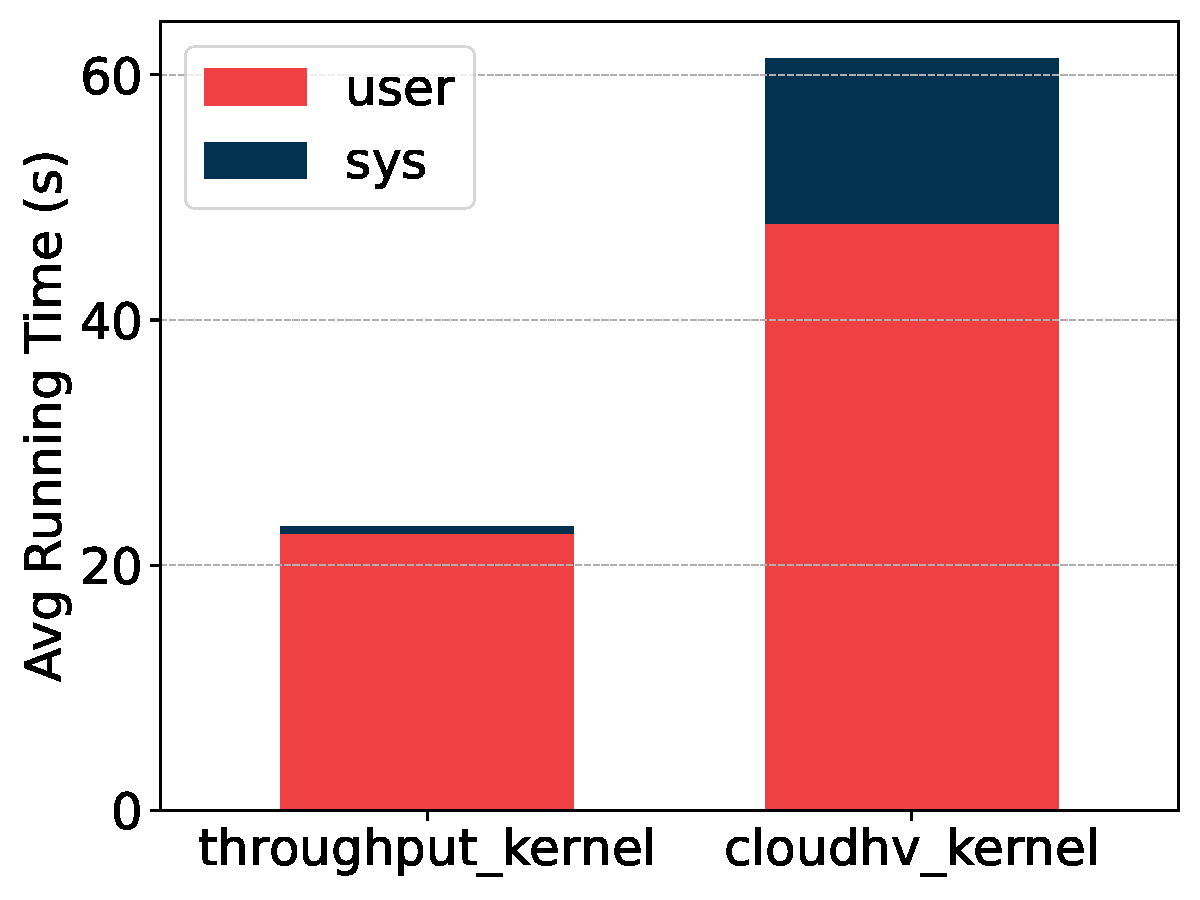
\includegraphics[width=\textwidth]{throughput_kernel_graph500}
        \caption{\quad Graph500平均运行时间}
        \label{fig:throughput_kernel_graph500}
    \end{subfigure}
    \begin{subfigure}[b]{0.35\textwidth}
        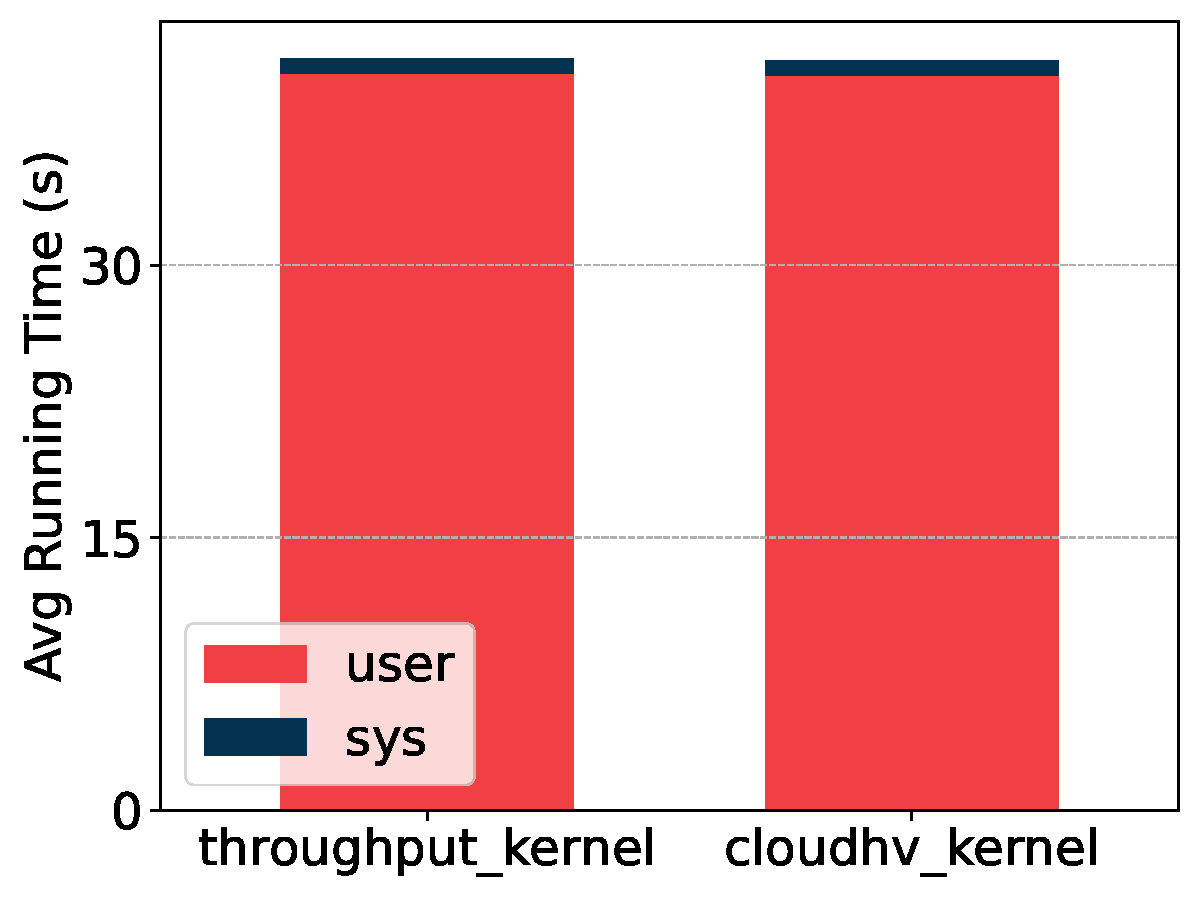
\includegraphics[width=\textwidth]{throughput_kernel_ffmpeg}
        \caption{\quad FFmpeg平均运行时间}
        \label{fig:throughput_kernel_ffmpeg}
    \end{subfigure}
    \bicaption{\quad 吞吐量优先内核对BE应用运行时间的影响}{\quad Impact of throughput-first kernel on BE application runtime}
    \label{fig:perf_throughput_time}
\end{figure}

\subsection{CPU资源感知策略效果}

% 普通场景
% 硬件场景:SMT

Control Tower CPU感知调度策略首先验证调度策略对高优先级任务的QoS保障能力,实验在4 CPU、1024 MB内存的虚拟机中展开,选择Redis、Memcached、Nginx与MySQL作为高优先应用来与stress\_ng CPU干扰混部,内核采用与CloudHV默认内核相同的HZ与抢占模式,并与CloudHV默认内核进行比较。

混部结果如图~\ref{fig:lc_bpf_sched}所示,总体来看,CPU资源感知调度策略几乎总是能够让LC应用达到与未受干扰情况下相近的性能。对于常见的LC应用Redis、Memcached与Nginx,CPU资源感知调度策略分别实现降低99分位尾延迟最高90.4\%、61.1\%、63.3\%的效果,同时在各个负载强度下均能有效保障应用的QoS。而对于业务逻辑较复杂的MySQL,CPU资源感知调度策略也同样能够很好地进行QoS保障,如图~\ref{fig:bpf_sched_smp_mysql}所示,在MySQL不同负载强度中,CPU感知调度策略实现了MySQL平均事务处理数量提升最高60.8\%的效果,同时请求延迟也最高降低了68.3\%。

\begin{figure}[H]
    \centering
    \begin{subfigure}[b]{0.32\textwidth}
        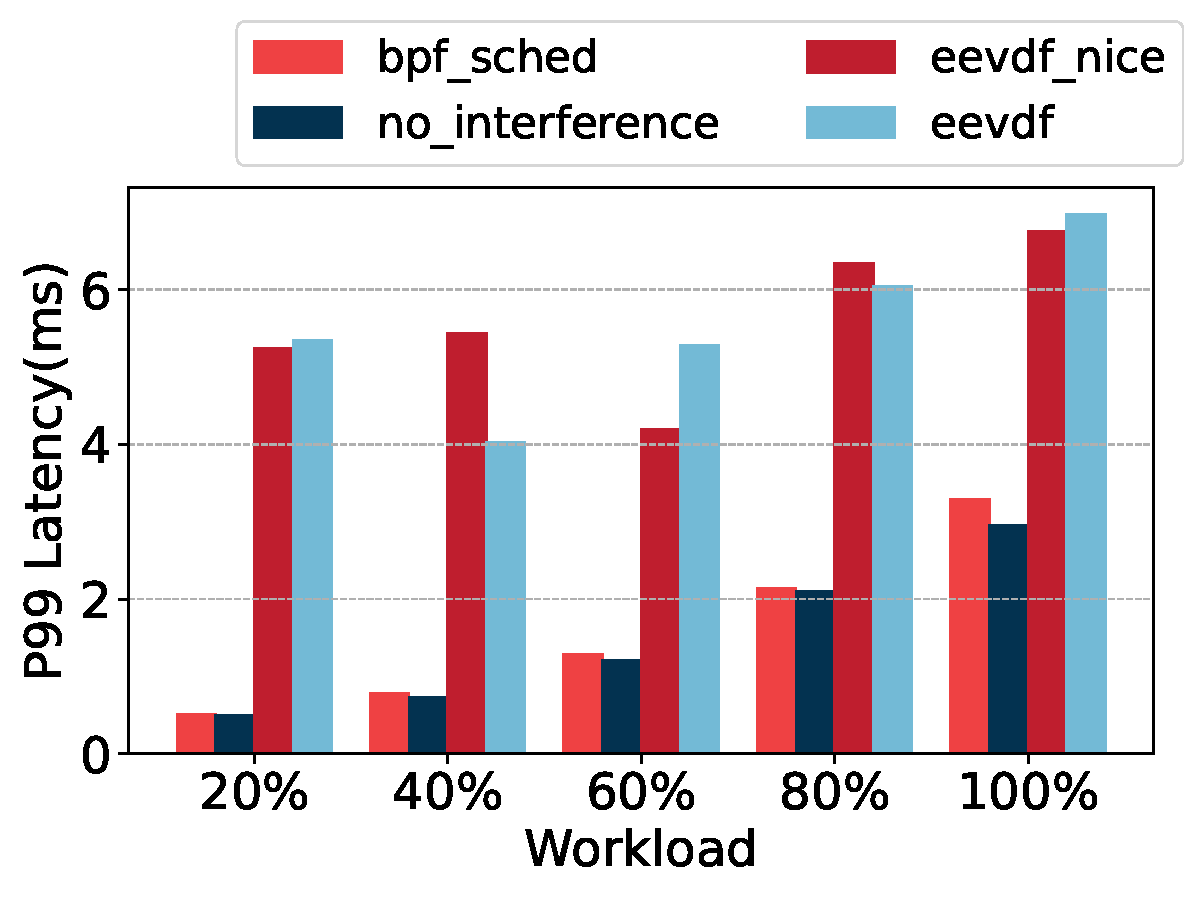
\includegraphics[width=\textwidth]{bpf_sched_smp_redis}
        \caption{\quad Redis请求延迟}
        \label{fig:bpf_sched_smp_memcached}
    \end{subfigure}
    \begin{subfigure}[b]{0.32\textwidth}
        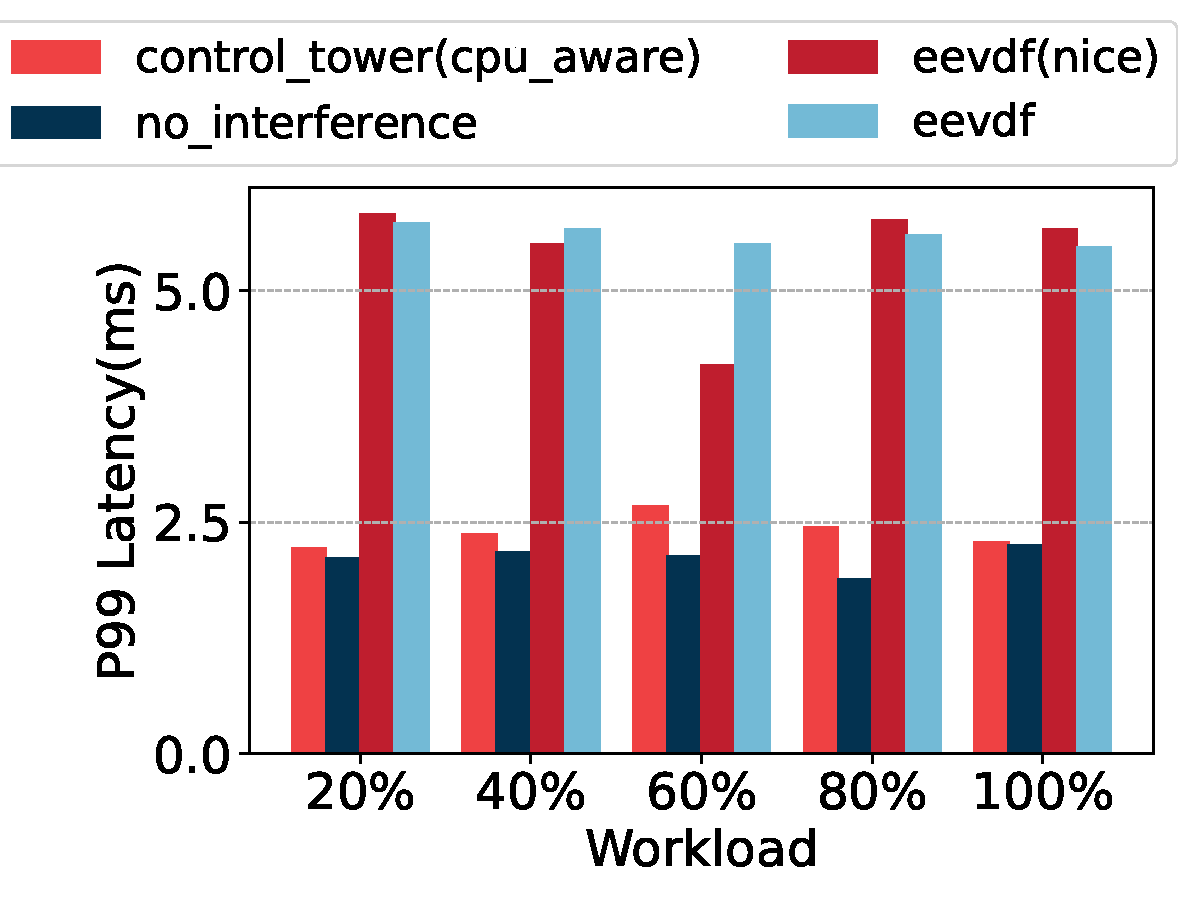
\includegraphics[width=\textwidth]{bpf_sched_smp_memcached}
        \caption{\quad Memcached请求延迟}
        \label{fig:bpf_sched_smp_memcached}
    \end{subfigure}
    \begin{subfigure}[b]{0.32\textwidth}
        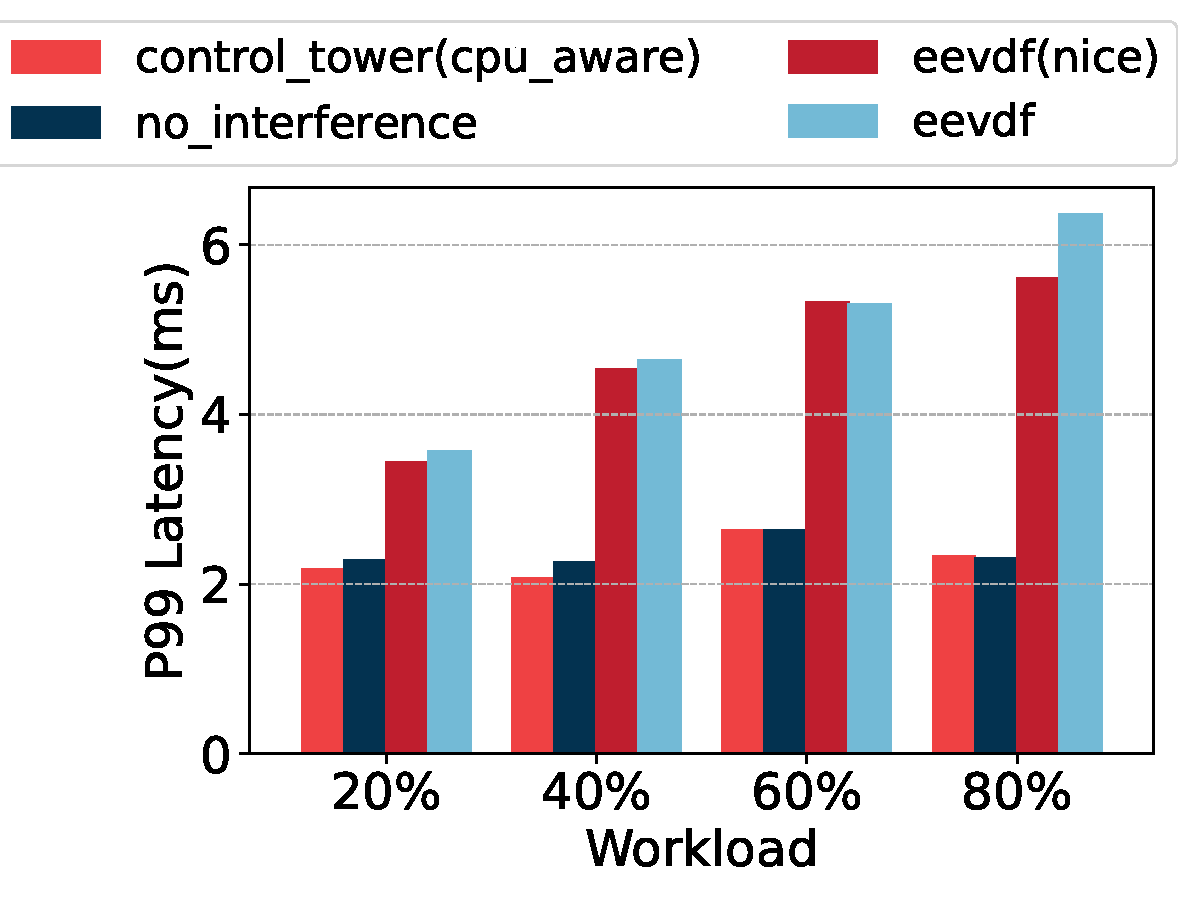
\includegraphics[width=\textwidth]{bpf_sched_smp_nginx}
        \caption{\quad Nginx请求延迟}
        \label{fig:bpf_sched_smp_memcached}
    \end{subfigure}
    \begin{subfigure}[b]{0.32\textwidth}
        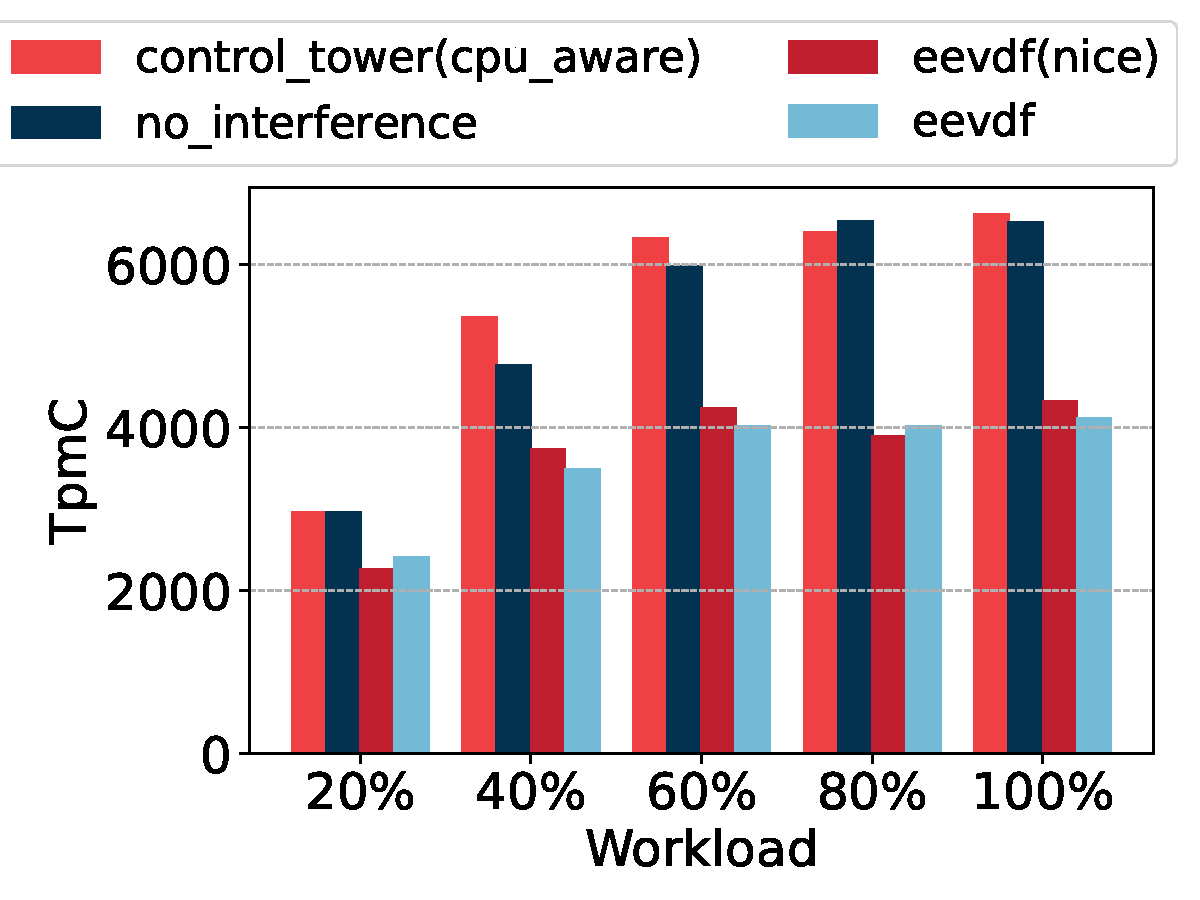
\includegraphics[width=\textwidth]{bpf_sched_smp_mysql}
        \caption{\quad MySQL每秒事务数量}
        \label{fig:bpf_sched_smp_mysql}
    \end{subfigure}
    \begin{subfigure}[b]{0.32\textwidth}
        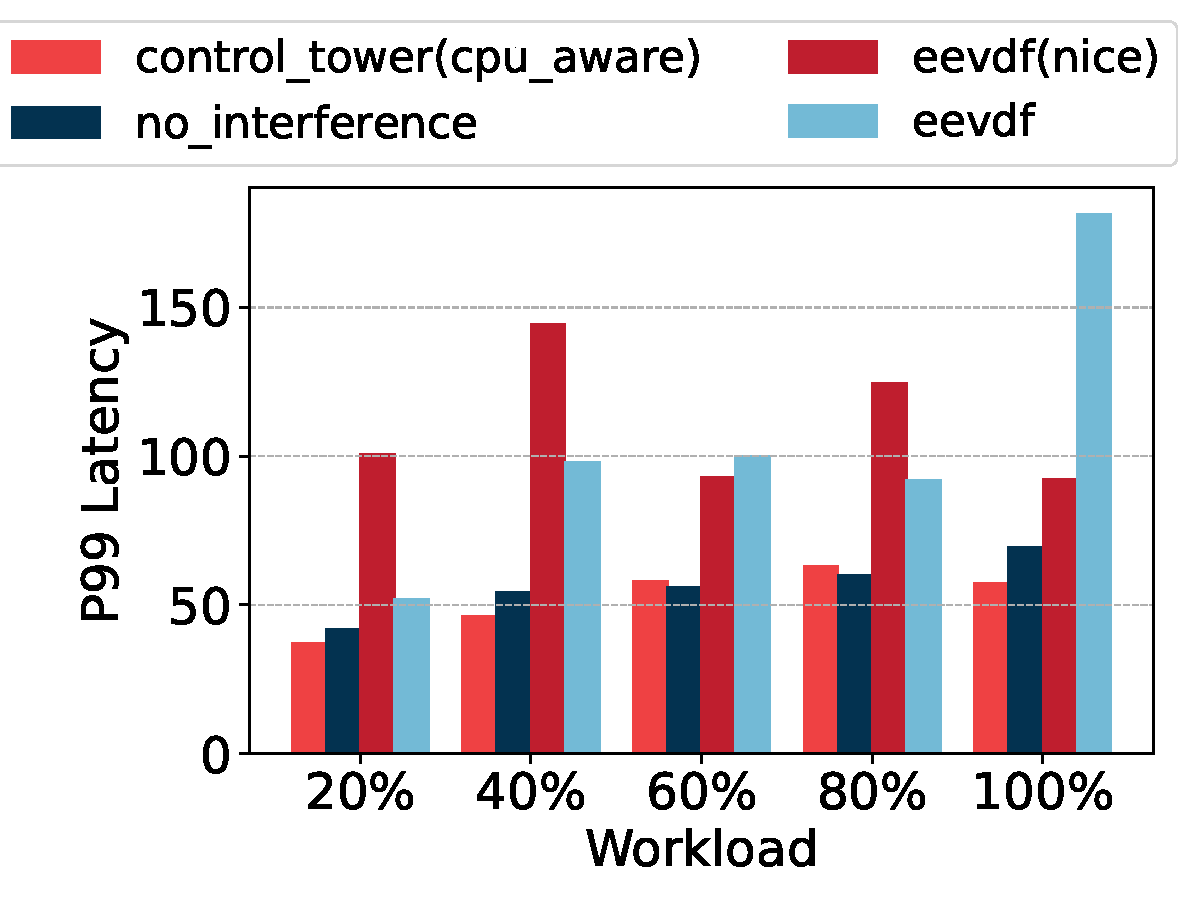
\includegraphics[width=\textwidth]{bpf_sched_smp_mysql_latency}
        \caption{\quad MySQL请求延迟} 
        \label{fig:bpf_sched_smp_mysql_latency}
    \end{subfigure}

\bicaption{\quad CPU感知调度策略对LC应用服务性能的保障效果}{\quad Effectiveness of CPU-aware scheduling policy for LC application QoS}
\label{fig:lc_bpf_sched}
\end{figure}

在总吞吐上,不同调度算法下的虚拟机的总CPU利用率如图~\ref{fig:cpu_usage}所示。其中,对于Redis、Memcached、Nginx而言,混部场景中总CPU几乎都完全占满。对比无干扰下的CPU利用率能够发现,额外的CPU资源占用由干扰应用产生,此时分配CPU资源的方式决定了混部场景下QoS保障的效果。

\begin{figure}[H]
    \centering
    \begin{subfigure}[b]{0.33\textwidth}
        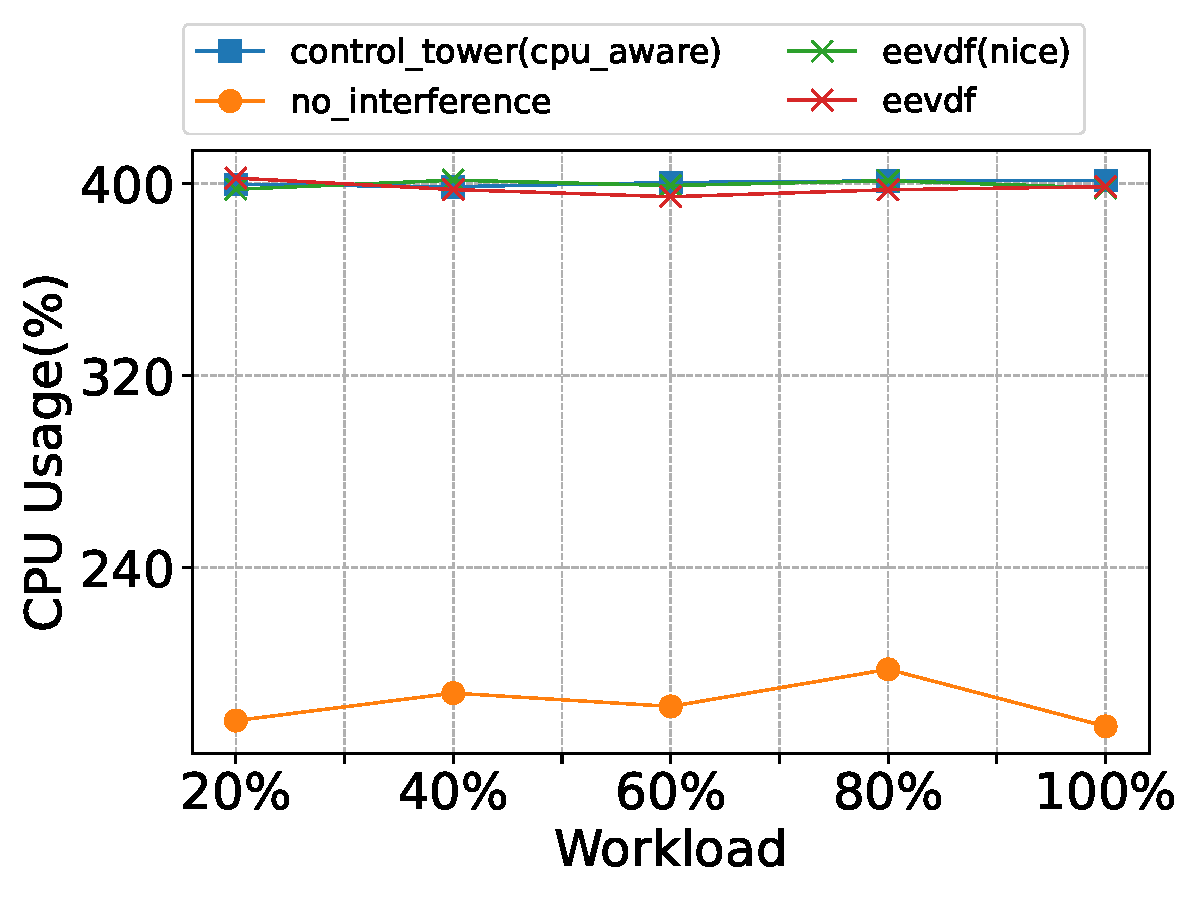
\includegraphics[width=\textwidth]{cpu_usage_redis}
        \caption{Redis-干扰}
        \label{fig:cpu_usage_redis}
    \end{subfigure}
    \begin{subfigure}[b]{0.33\textwidth}
        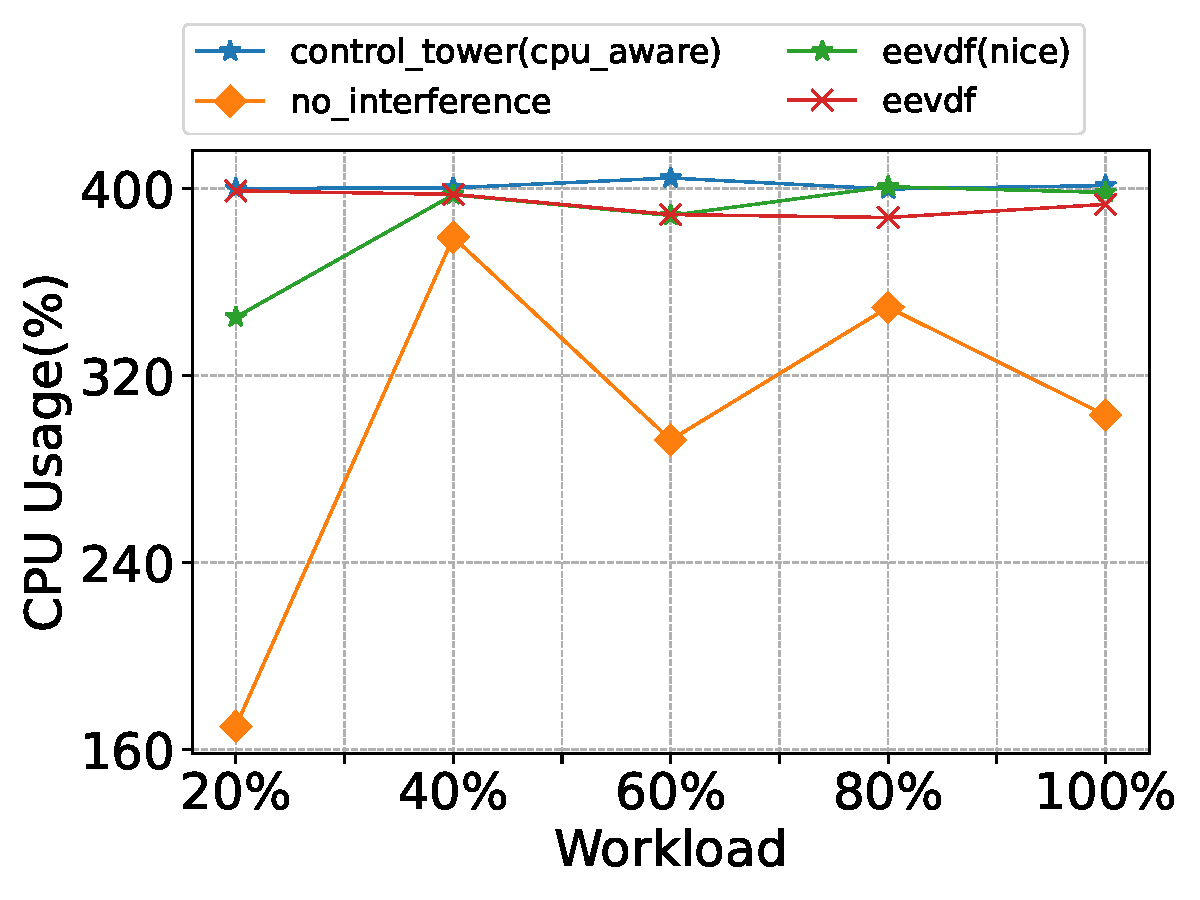
\includegraphics[width=\textwidth]{cpu_usage_memcached}
        \caption{Memcached-干扰}
        \label{fig:cpu_usage_memcached}
    \end{subfigure}
    \begin{subfigure}[b]{0.33\textwidth}
        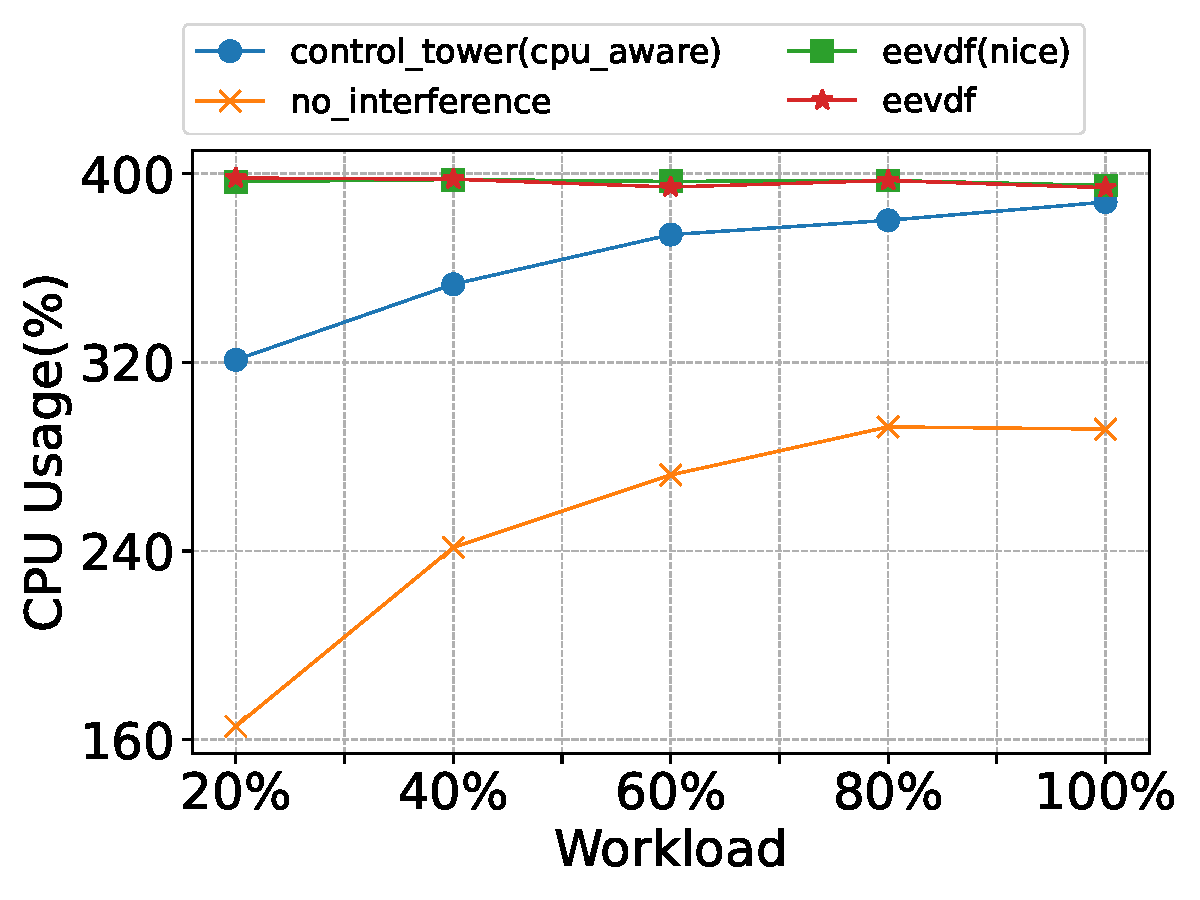
\includegraphics[width=\textwidth]{cpu_usage_mysql}
        \caption{MySQL-干扰}
        \label{fig:cpu_usage_mysql}
    \end{subfigure}
    \begin{subfigure}[b]{0.33\textwidth}
        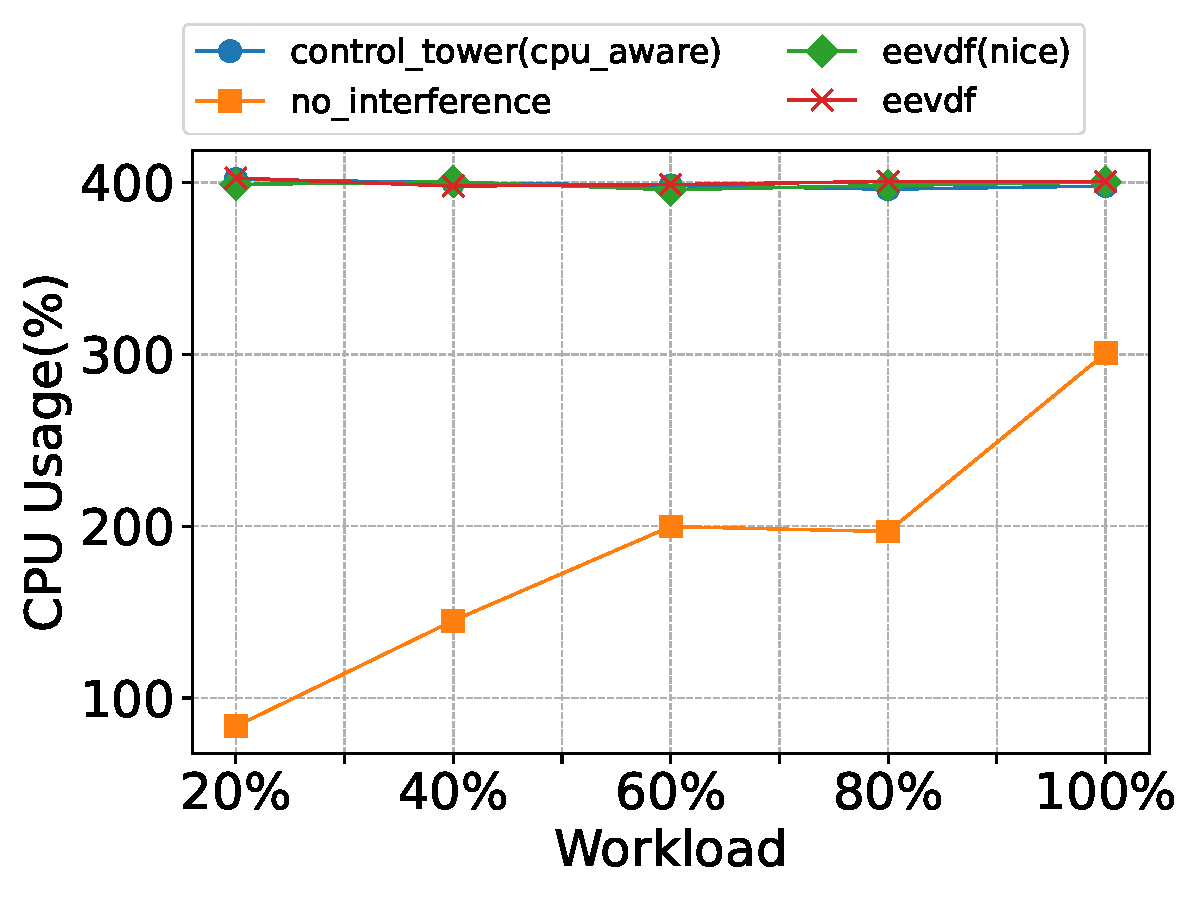
\includegraphics[width=\textwidth]{cpu_usage_nginx}
        \caption{Nginx-干扰}
        \label{fig:cpu_usage_nginx}
    \end{subfigure}
\bicaption{\quad 不同应用混部时虚拟机总CPU利用率}{\quad 
Total CPU utilization of virtual machines with different co-location applications}
\label{fig:cpu_usage}
\end{figure}

相较于Linux任务调度机制,CPU感知调度策略能够做到更好的QoS保障效果,核心原因在于合理地CPU资源分配。CPU感知调度策略基于Control Tower任务调度框架设计,使得低优先任务总是能够在高优先应用需要时及时地出让CPU资源,并在高优先应用运行的过程中确保不进行抢占,从而实现更好的QoS保障效果。

混部场景中调度需要考虑硬件的特性,如SMT中兄弟核心之间存在片上共享资源,Linux任务调度策略中的措施是通过调度域名尽量避免将任务调度到SMT上,但这种做法并不能充分利用SMT资源。造成上述问题的核心在于缺少一种CPU感知的机制,让SMT调度时知道兄弟核心的运行情况,而CPU感知调度策略恰好能够解决这一问题。

混部实验在2 SMT CPU、1024 MB内存的虚拟机中展开,选择Redis、Memcached、Nginx、MySQL四种延时敏感应用与stress\_ng CPU干扰进行混部。实验结果如图~\ref{fig:lc_bpf_sched_smt}所示,相较于EEVDF,CPU感知调度策略能够在所测应用的各个负载下有效地对应用QoS进行保障。其中对于Redis、Memcached、MySQL,CPU感知调度策略分别实现了99分位尾延迟降低最高71.2\%、48.7\%、49.5\%的效果。特别地,Nginx在高负载时由于SMT场景的激烈资源竞争,Linux EEVDF调度器几乎无法进行有效调度,导致Nginx延时呈数量级的上升,而在该场景下,如图~\ref{fig:bpf_sched_smt_nginx}所示,CPU感知调度策略则仍然能够实现Nginx与无干扰类似的性能表现。

\begin{figure}[H]
    \centering
    \begin{subfigure}[b]{0.32\textwidth}
        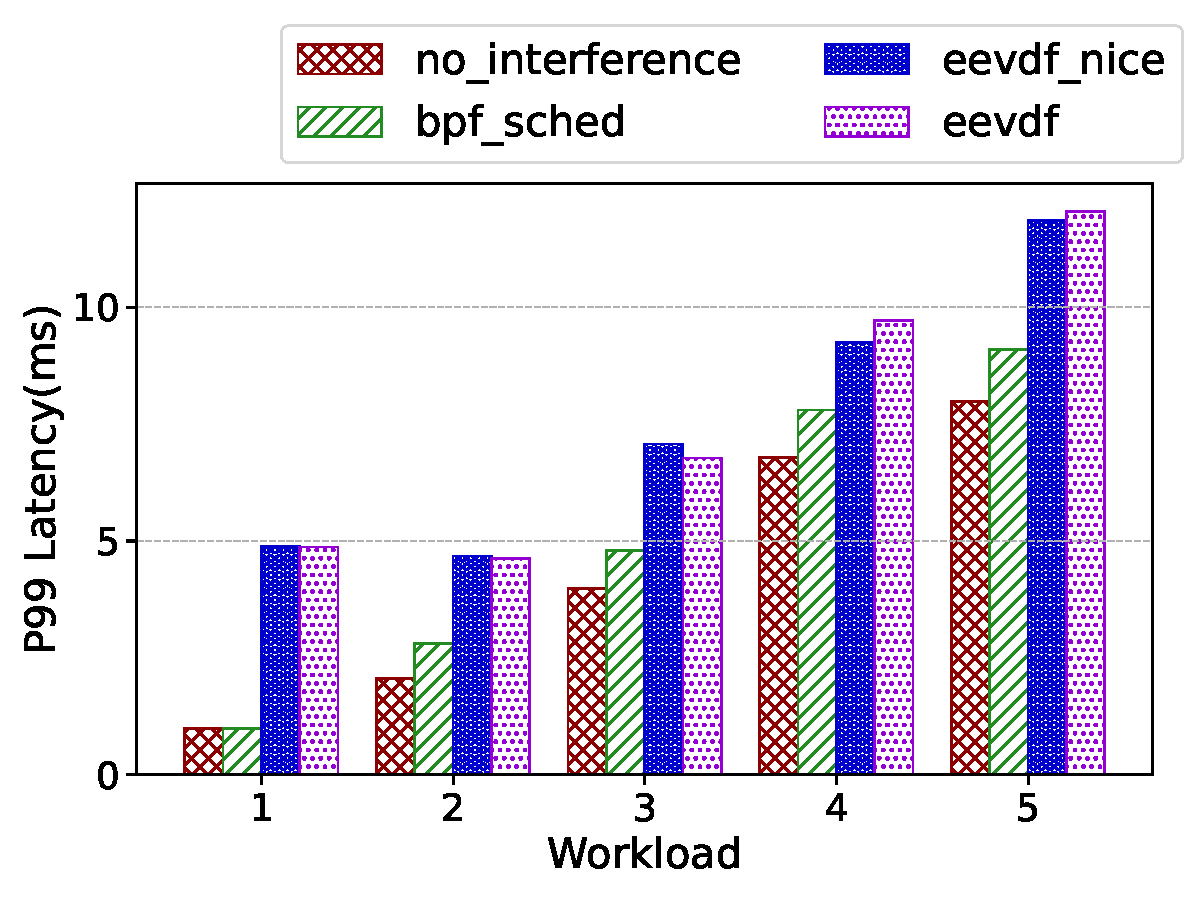
\includegraphics[width=\textwidth]{bpf_sched_smt_redis}
        \caption{\quad Redis请求延迟}
        \label{fig:bpf_sched_smt_redis}
    \end{subfigure}
    \begin{subfigure}[b]{0.32\textwidth}
        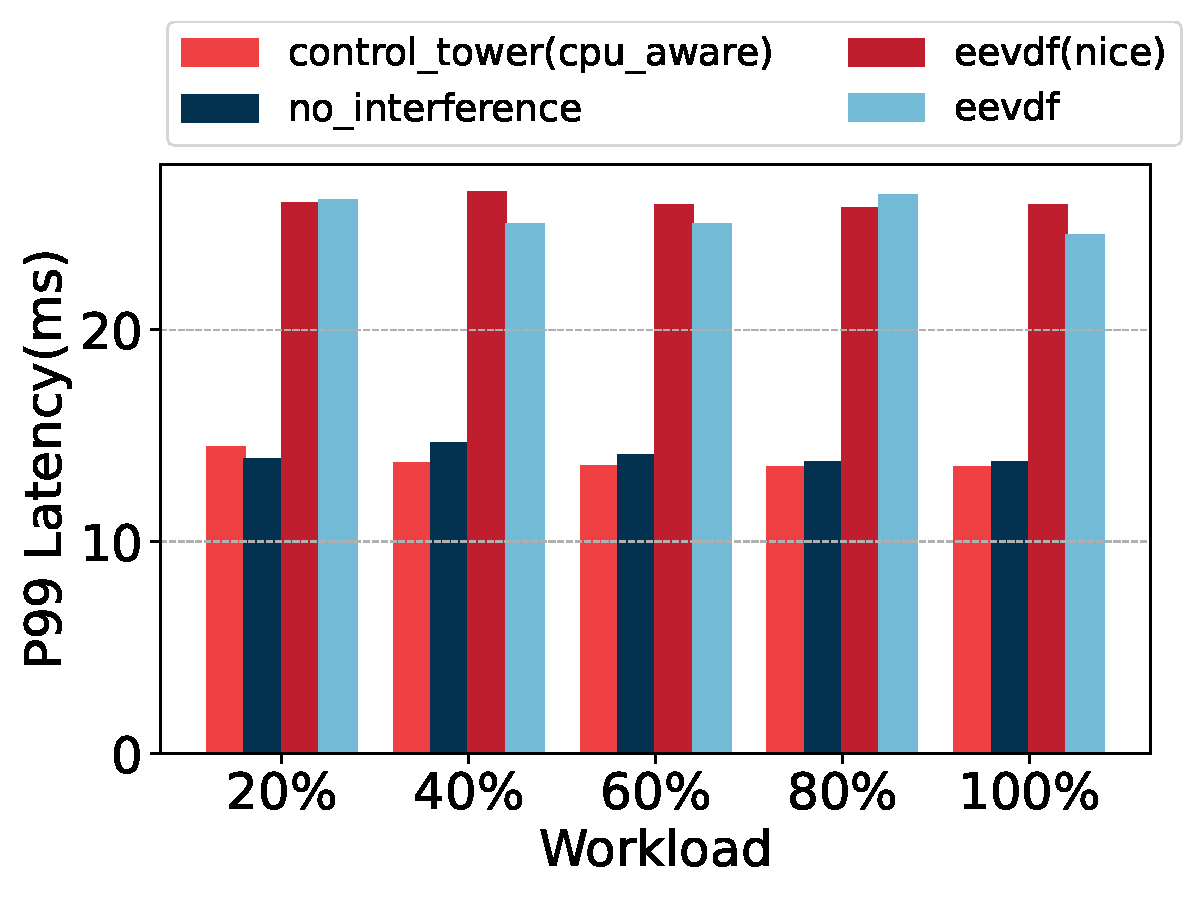
\includegraphics[width=\textwidth]{bpf_sched_smt_memcached}
        \caption{\quad Memcached请求延迟}
        \label{fig:bpf_sched_smt_memcached}
    \end{subfigure}
    \begin{subfigure}[b]{0.32\textwidth}
        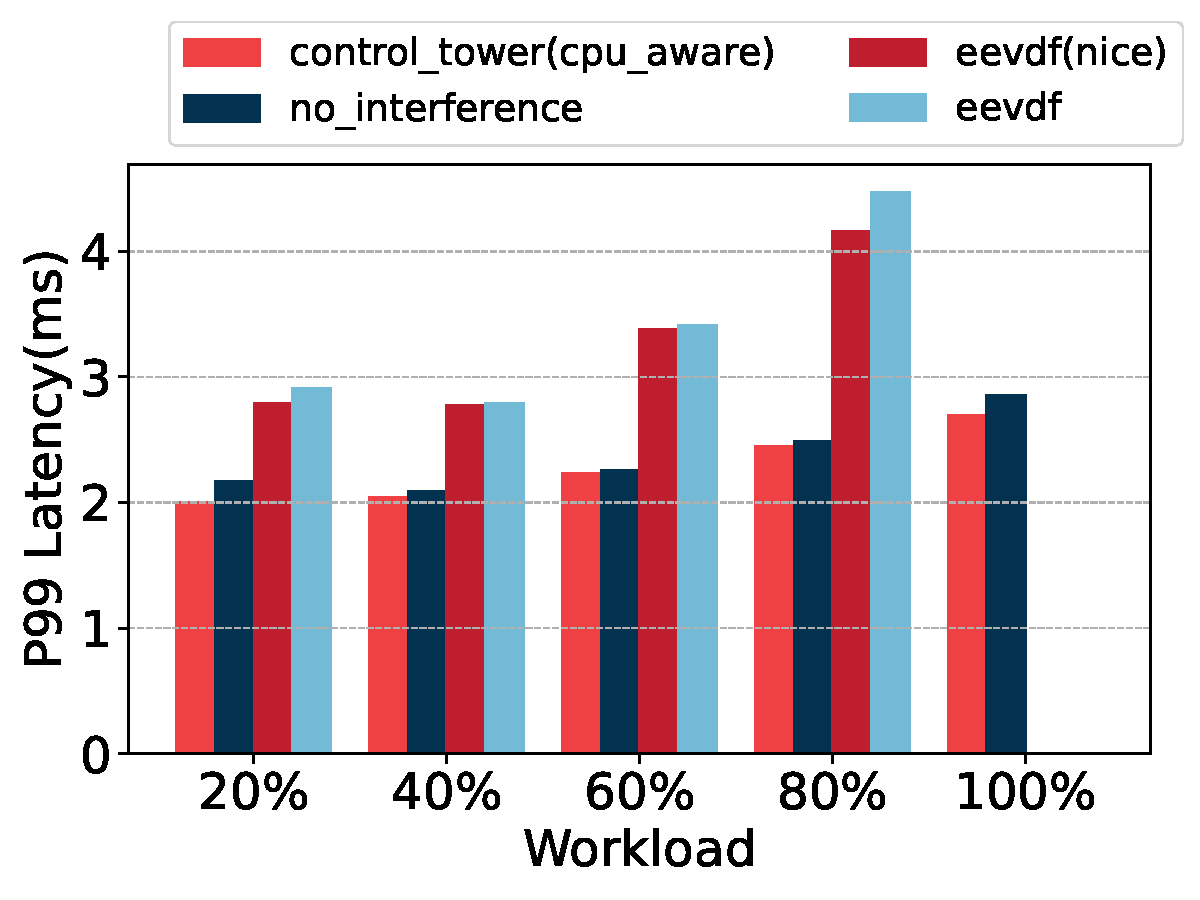
\includegraphics[width=\textwidth]{bpf_sched_smt_nginx}
        \caption{\quad Nginx请求延迟}
        \label{fig:bpf_sched_smt_nginx}
    \end{subfigure}
    \begin{subfigure}[b]{0.32\textwidth}
        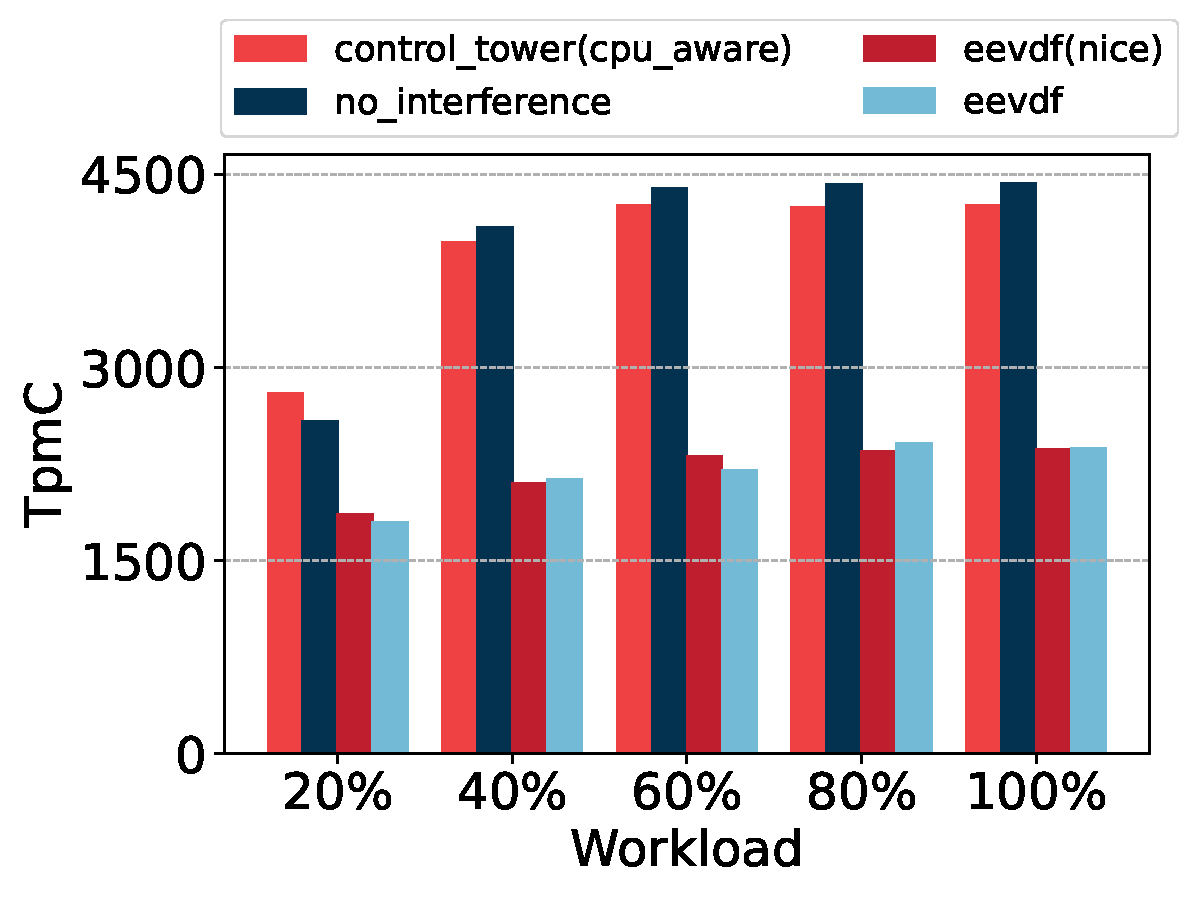
\includegraphics[width=\textwidth]{bpf_sched_smt_mysql}
        \caption{\quad MySQL每秒事务数量}
        \label{fig:bpf_sched_smt_mysql}
    \end{subfigure}
    \begin{subfigure}[b]{0.32\textwidth}
        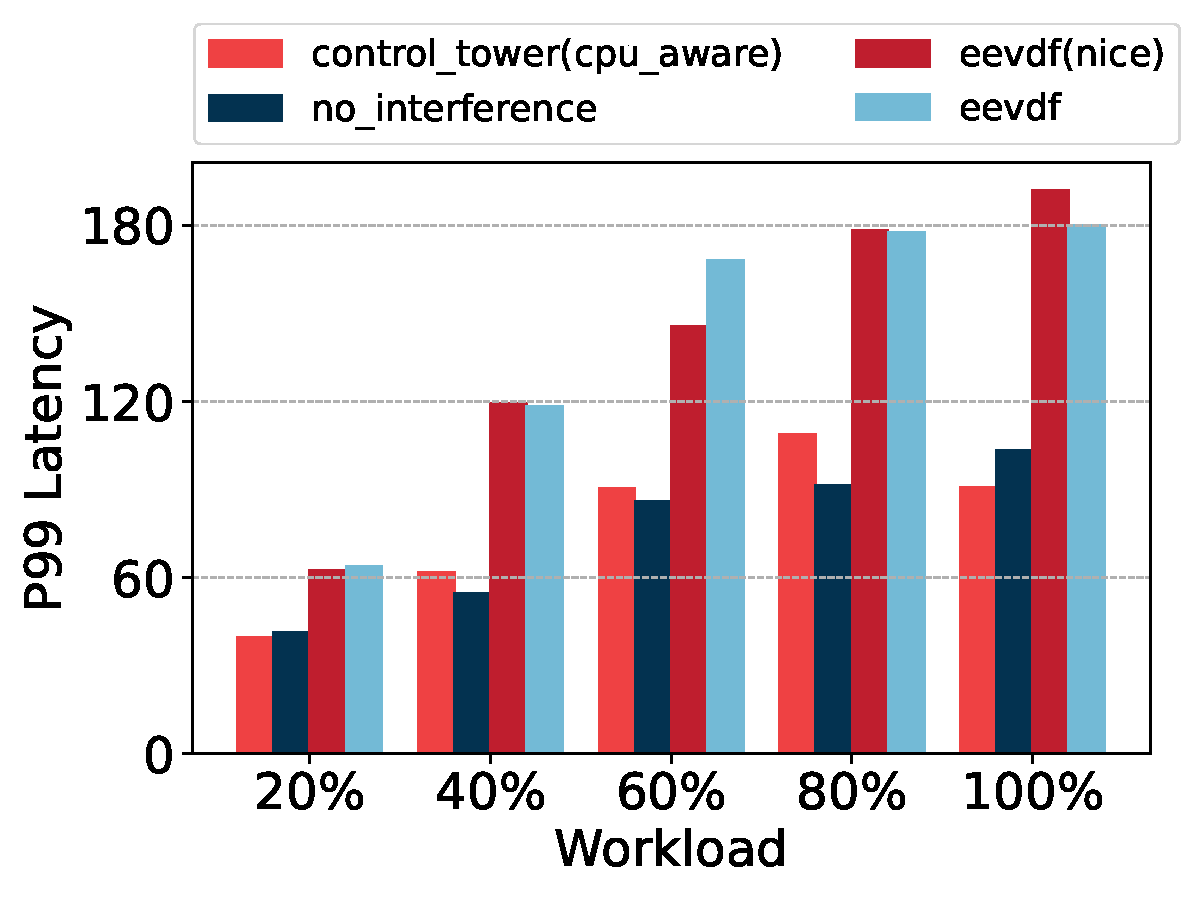
\includegraphics[width=\textwidth]{bpf_sched_smt_mysql_latency}
        \caption{\quad MySQL请求延迟}
        \label{fig:bpf_sched_smt_mysql_latency}
    \end{subfigure}
\bicaption{\quad SMT场景下CPU感知调度策略对LC应用服务性能的保障效果}{\quad Effectiveness of CPU-aware scheduling policy for LC application QoS on SMT}
\label{fig:lc_bpf_sched_smt}
\end{figure}

Control Tower CPU感知调度策略在保障延时的同时,同时也保障了延时的稳定度,这点对于LC应用而言也十分重要。以Redis为例,如图~\ref{fig:latency_box}所示,在CPU感知调度策略下,Redis的各个负载下的延时波动都几乎与无干扰状态下相同。

\begin{figure}[H]
    \centering
    \begin{subfigure}[b]{0.35\textwidth}
        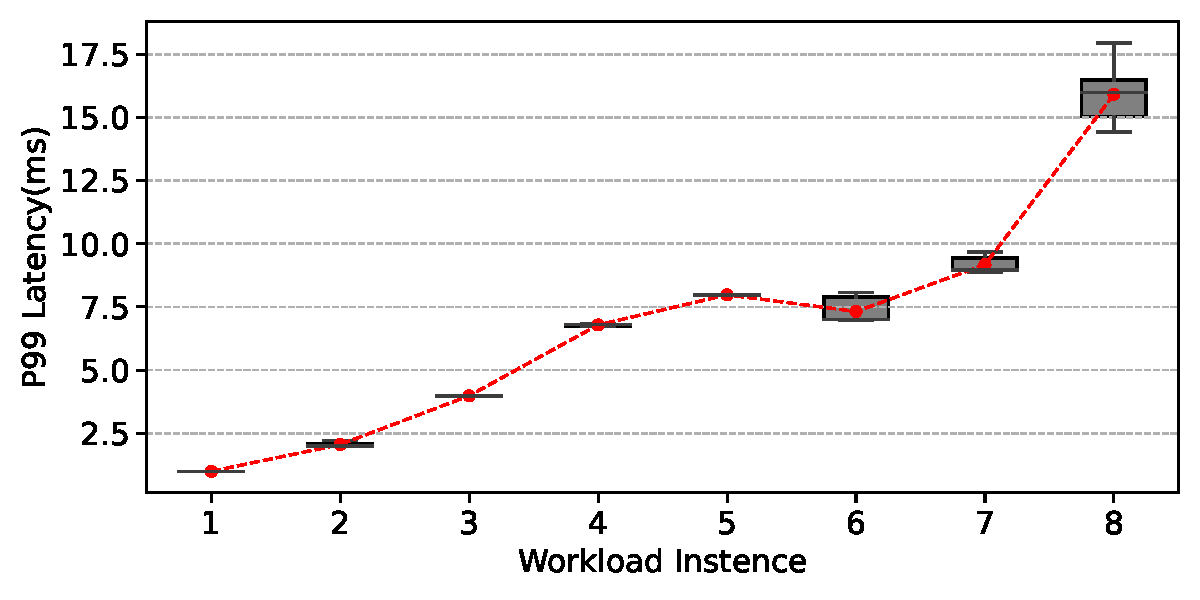
\includegraphics[width=\textwidth]{cpu_aware_box_no_interference}
        \caption{无干扰场景}
        \label{fig:cpu_aware_box_no_interference}
    \end{subfigure}
    \begin{subfigure}[b]{0.35\textwidth}
        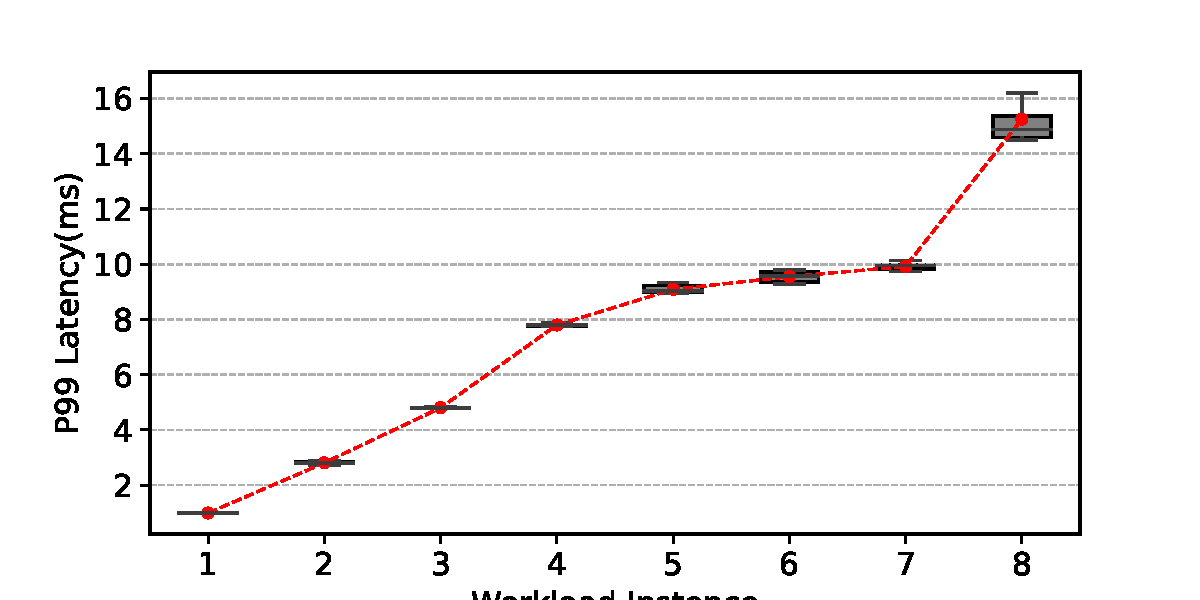
\includegraphics[width=\textwidth]{cpu_aware_box_bpf_sched}
        \caption{CPU感知调度策略}
        \label{fig:cpu_aware_box_bpf_sched}
    \end{subfigure}
    \begin{subfigure}[b]{0.35\textwidth}
        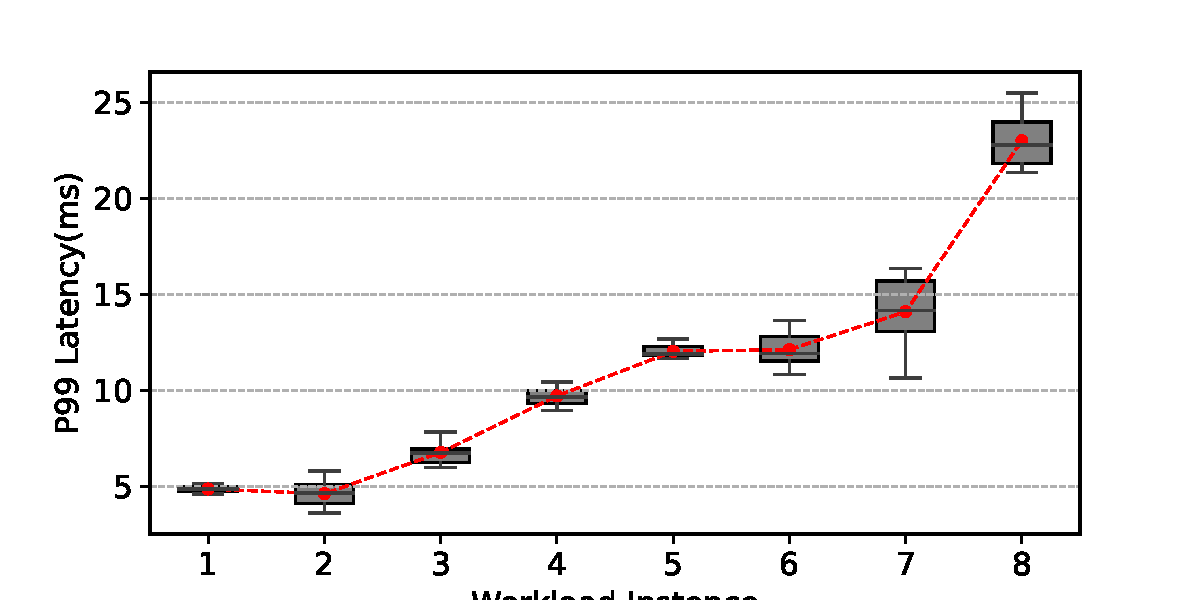
\includegraphics[width=\textwidth]{cpu_aware_box_eevdf}
        \caption{EEVDF调度器}
        \label{fig:cpu_aware_box_eevdf}
    \end{subfigure}
    \begin{subfigure}[b]{0.35\textwidth}
        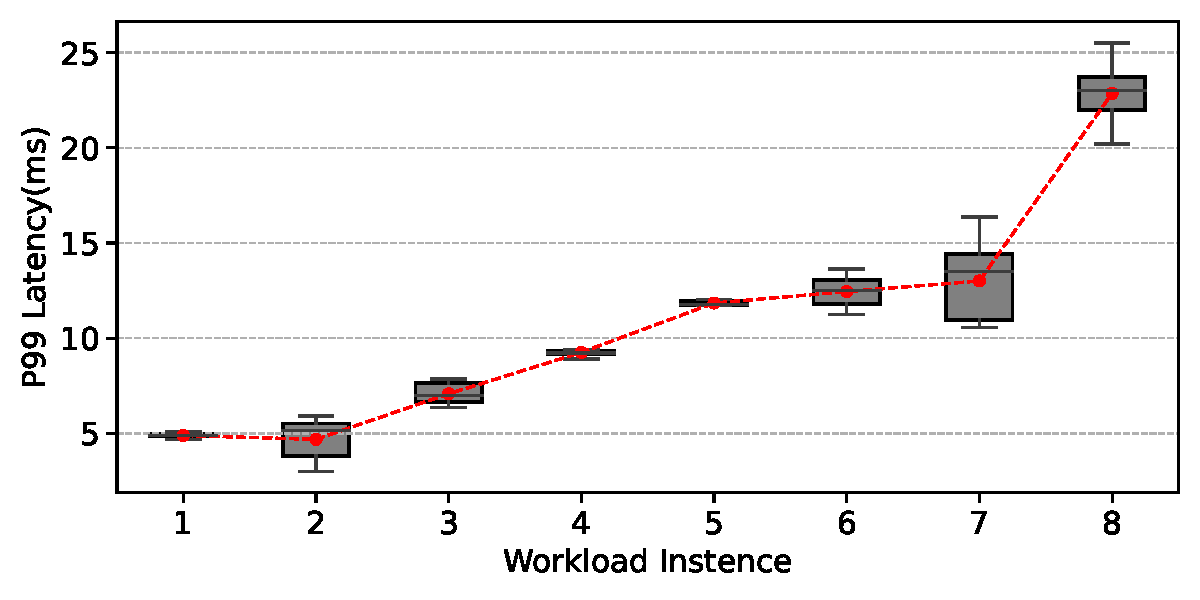
\includegraphics[width=\textwidth]{cpu_aware_box_eevdf_nice}
        \caption{EEVDF高优先级}
        \label{fig:cpu_aware_box_eevdf_nice}
    \end{subfigure}
\bicaption{\quad SMT下不同调度策略对Redis延迟稳定性的影响}{\quad The impact of different scheduling strategies on Redis latency stability on SMT}
\label{fig:latency_box}
\end{figure}

实现这一延时保障效果的核心原因在于Control Tower任务调度框架中的eBPF数据源与BPF调度策略都完全运行在内核态,并借助内核提供的数据结构交互,因此在调度决策上速度上能够做到与内核调度周期同步,从而避免了许多用户态调度器因调度延时较大所导致的决策与实时资源分配偏差的问题。

\subsection{网络资源感知策略效果}

Control Tower网络资源感知调度策略实验在一个4CPU、1024MB内存的虚拟机展开。首先,截取Redis、Memcached、Nginx与Mysql四个常见网络服务型应用在一段时间内的负载与epoll时间计数。如图~\ref{fig:epoll_request}所示,对于Redis、Memcached、Nginx三种应用而言,epoll wait返回的事件数量与请求量高度相关,而考虑epoll事件的统计发生在服务端,而请求数量的统计发生在客户端,因此两端序列在时间上存在一定的偏移。然而,对于没有使用epoll作为底层网络机制实现的MySQL,这种监测方式就不能反映应用的网络资源使用,需要依赖其他的手段。由此也反映出,在不同的混部场景下对监测手段的要求也不同。

\begin{figure}[!htbp]
    \centering
    \begin{subfigure}[b]{0.49\textwidth}
        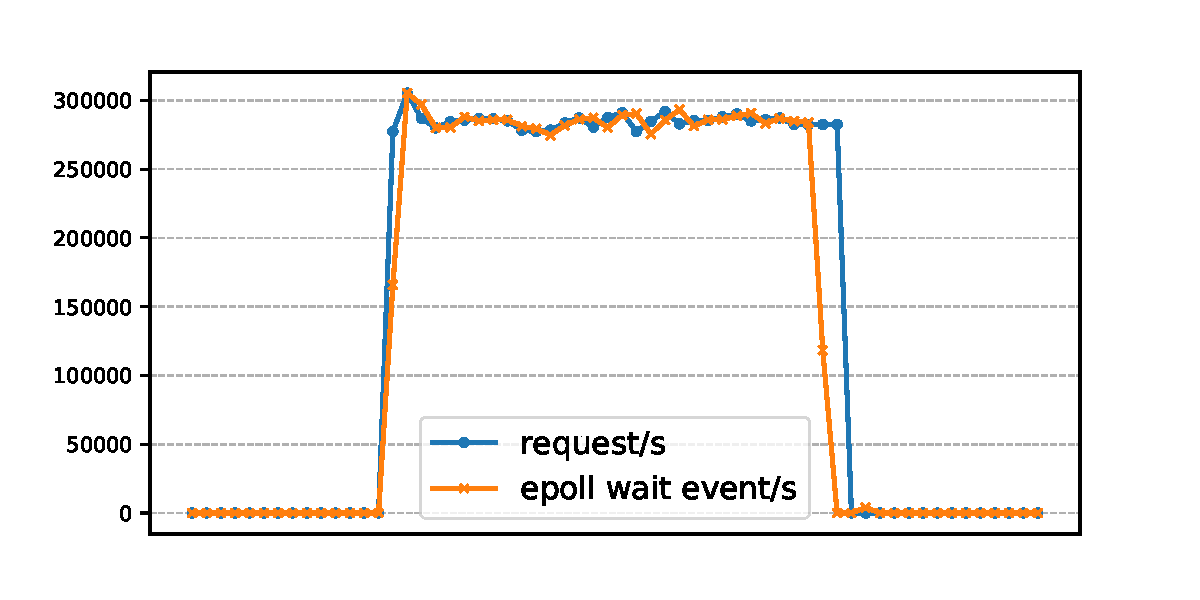
\includegraphics[width=\textwidth]{epoll_memcached}
        \caption{Memcached请求数量与Epoll Wait事件数量}
        \label{fig:epoll_memcached}
    \end{subfigure}
    \begin{subfigure}[b]{0.49\textwidth}
        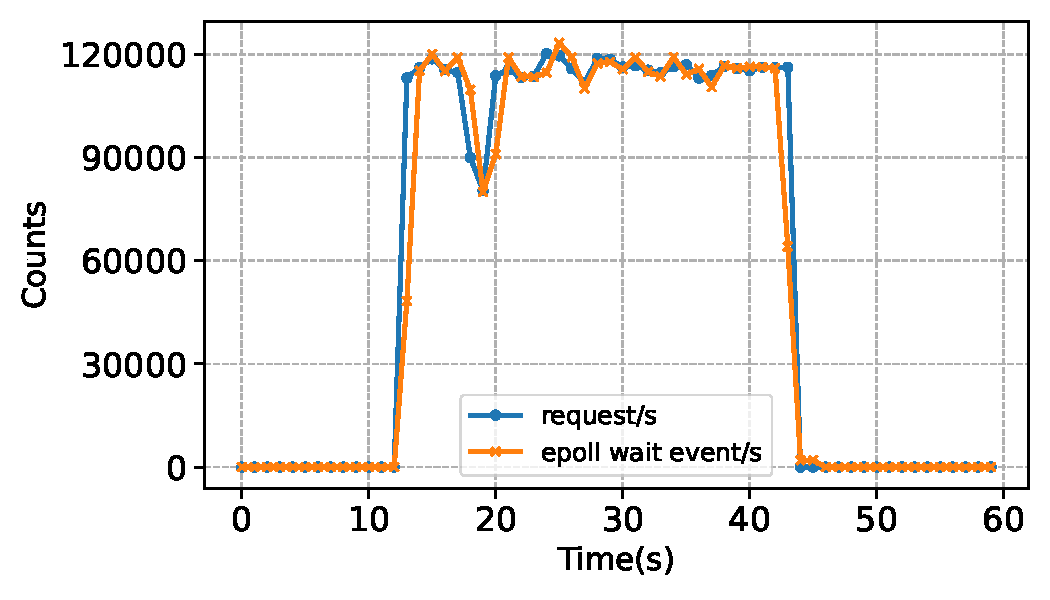
\includegraphics[width=\textwidth]{epoll_redis}
        \caption{Redis请求数量与Epoll Wait事件数量}
        \label{fig:epoll_redis}
    \end{subfigure}
    \begin{subfigure}[b]{0.49\textwidth}
        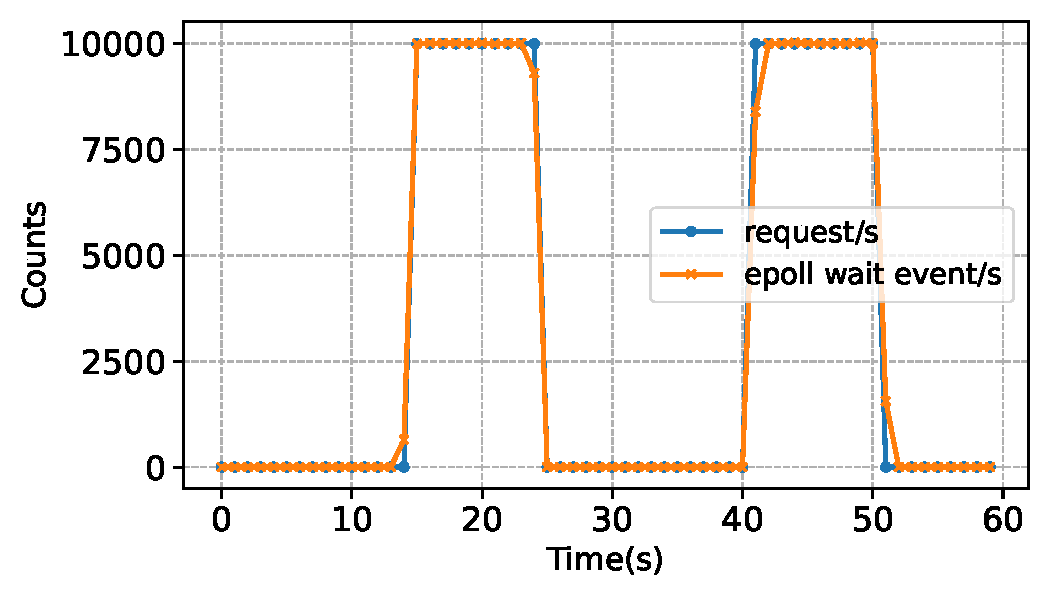
\includegraphics[width=\textwidth]{epoll_nginx}
        \caption{Nginx请求数量与Epoll Wait事件数量}
        \label{fig:epoll_nginx}
    \end{subfigure}
    \begin{subfigure}[b]{0.49\textwidth}
        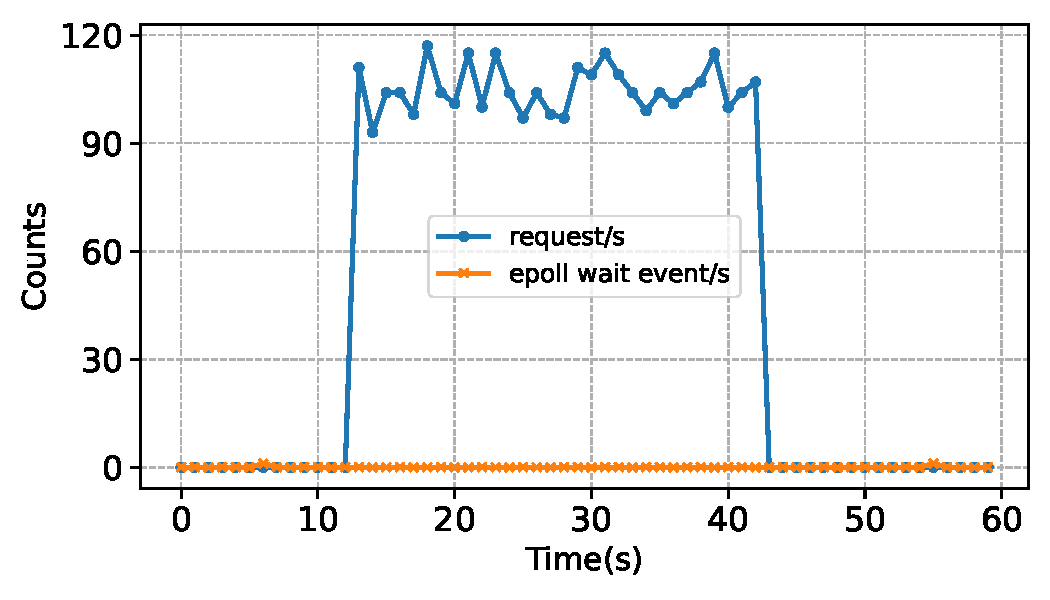
\includegraphics[width=\textwidth]{epoll_mysql}
        \caption{Mysql请求数量与Epoll Wait事件数量}
        \label{fig:epoll_mysql}
    \end{subfigure}
\bicaption{\quad LC应用负载与Epoll Wait事件数量的关系}{\quad The relationship between LC application workloads and epoll Wait events}
\label{fig:epoll_request}
\end{figure}

网络资源感知策略下的混部实验选择Nginx作为LC应用,并将其最大负载的20\%作为调度的临界值。混部结果如图~\ref{fig:network_aware_cpu_usage}所示,其中红色虚线部分标注了调度策略的负载临界值。时序图中,Nginx负载不断增加,同时CPU占用率也有所上升,在临界值之前,由于调度策略较宽松,整体调度以吞吐量为目标,因此系统总CPU利用率接近100\%,而随负载的不断增加,应用间CPU资源争抢越来越激烈,整体CPU资源波动较大。临界值之后,调度策略转变为以保障LC应用延时为目标,并开始严格限制低优先任务的CPU资源使用。此时虽然整体CPU利用率随Nginx负载增大而有所降低,但整体CPU利用率波动变得更小,同时也保障了Nginx的QoS。

\begin{figure}[H]
    \centering
    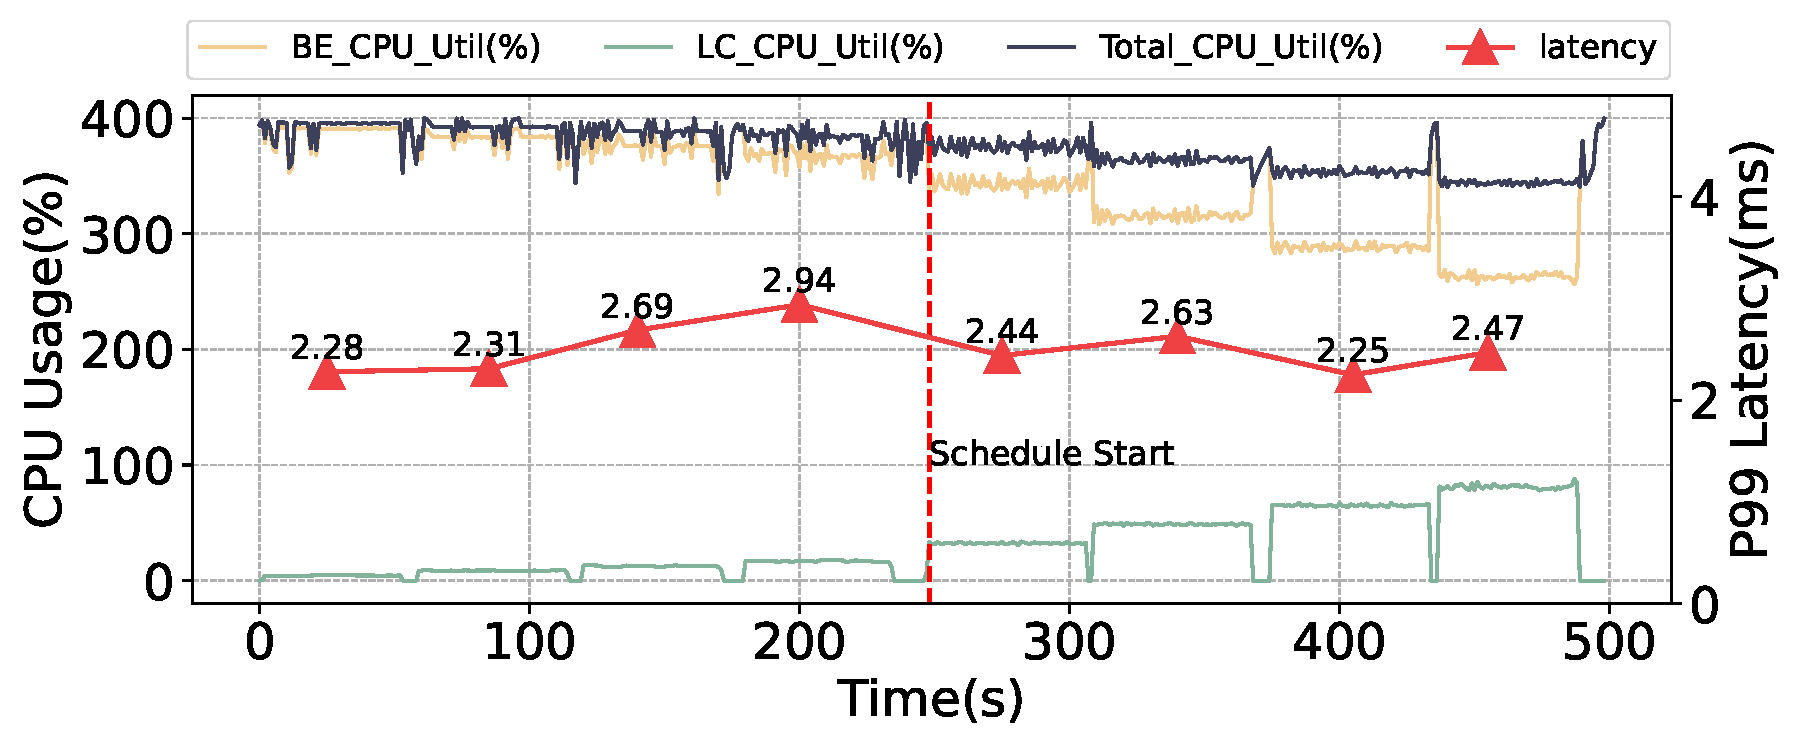
\includegraphics[width=0.9\textwidth]{network_aware_cpu_usage}
    \bicaption{\quad 应用与干扰混部一段时间内的CPU使用率}{\quad The CPU utilization of applications and interference over a period of time}
    \label{fig:network_aware_cpu_usage}
\end{figure}

% \subsection{内存资源感知策略}
% Redis

\section{本章小结}

本章首先针对画像分析中不同类型应用,基于内核中关于HZ与抢占模型的配置,设计了调度配置的定制优化,提供了吞吐量优先与响应度优先两种不同调度目标的内核配置。

随后,为解决混部场景下,Linux任务调度机制调节手段单一、优先性存在缺陷的问题,设计实现了Control Tower任务调度框架。框架基于Sched Ext项目实现,首先,框架允许通过用户输入与eBPF插桩,为调度策略提供丰富的决策信息。其次,框架借助Ext调度类的优先级特点,实现任务的全局高优先性。最后,框架利用BPF调度策略的灵活性,能够针对不同的混部场景,定制混部任务所需的调度方式。

在Control Tower任务调度框架的基础上,本文进一步设计了CPU感知的任务调度策略与网络资源感知的任务调度策略。其中,CPU感知任务调度策略通过感知高优先任务的CPU资源使用情况,结合用户定义的CPU阈值,在利用系统中的空闲CPU资源的同时,也能结合混部场景中CPU资源的不同特性来快速地向高优先任务出让CPU资源,从而实现有效的QoS保障。网络资源感知调度策略则通过监听epoll\_wait系统调用,了解系统中网络应用的负载情况,并适时地调整调度策略,以便于在网络应用的不同负载下进行区别性地管理。

本章实验中,首先围绕内核任务调度配置在虚拟化环境中展开实验。其中,响应度优先内核能够在混部场景下,能够最高降低LC应用39.2\%的延迟。吞吐量优先内核则能够在混部场景下,最高提升应用165.2\%的执行速度。随后,在Control Tower任务调度框架的实验中,CPU感知调度策略能够在混部实验中,相较于Linux任务调度实现90.4\%的延迟降低效果,并在混部任务的的各个负载下,是其接近于单独部署时的性能。除此之外,CPU感知调度策略也能够很好的解决SMT混部场景下的调度问题。